\chapter{Sorterede følger}
\renewcommand{\labelprefix}{ch:search}
\llabel{}
\vspace*{-4.5cm}
\begin{flushright}
%\psfrag{00}{$\infty$}
%\includegraphics[scale=0.5]{img/cloud2.eps}
\includegraphics[width=5cm]{img/KarteikastenKlein.eps}
\end{flushright}
\vspace*{0.5cm}

{\textit\noindent 
Vi tilbringer alle en betydelig del af vores tid med at lede efter ting.
\index{søgning|textbf}
Sådan er det også med datamater:
De slår op efter telefonnumre, saldoer, flyreservationer, regninger og betalinger, osv.
I mange anvendelser skal der søges i dynamiske, dvs. foranderlige, datamængder.
Nye reservationer føjer til reservationssystemet, reservationer ændres eller slettes, og reservationer bliver til faktisk gennemførte flyafgange.
Vi har allerede mødt én løsning på dette problem, nemlig hachning. hadsning. hasning. hashning, hashing.
Men ofte ønsker vi at holde den foranderlige datamængde i sorteret orden.
For at sikre denne tilstand manuelt benytter man et kartotek.
\index{kartotek}
Nye kartotekskort kan indsættes, fjernes,
% TODO orig confusing: an jeder beliebigen Position depends on sorted order
kortene kan gennemses i sorteret rækkefølge og man kan bruge en slags binærsøgning for at finde et bestemt kort.
I gamle date bestod kartotekssystemet af store biblioteker af hundretusindvis af kort.\footnote{Fotografiet viser kartotekskort i universitetsbiblioteket i Graz.  (Dr. M. Gossler).}}

\bigskip

I dette kapitel drejer det sig om at forvalte en mængde $S$ af indgange.
Hver indgang $e$ har en nøgle $\Id{nøgle}(e)$ taget fra en mængde \Id{Nøgle}, som er forsynet med en lineær ordning.
Dette definerer en rækkefølge på $S$.
Ved siden af søgning vil vi også støtte operationer til tilføjelse og fjernelse.
Dette fører til følgende grundoperationer på en
\emph{sorteret følge}
\index{sorteret følge|textbf}
\index{følge!sorteret|\siehe{sorteret følge}}
\index{søgetræ|siehe{sorteret følge}}
\index{sorteret følge!lokaliser@\Id{lokaliser}|textbf}
\index{sorteret følge!tilføj@\Id{tilføj}|textbf}
\index{sorteret følge!fjern@\Id{fjern}|textbf}
$S$: 
\begin{description}
\item[$S.\Id{lokaliser}(k:\Id{Nøgle})$:]
Returner indgangen med den mindste nøgle i $\{\,e\in S\colon\Id{nøgle}(e)\geq k\,\}$. 
\item[$S.\Id{tilføj}(e : \Id{Element})$:]
Hvis der findes $e'\in S$ med $\Id{nøgle}(e')=\Id{nøgle}(e)$, så $S\Is (S\setminus\set{e'})\cup\set{e}$.
     Ellers  $S\Is S\cup\set{e}$.
\item[$S.\Id{fjern}(k : \Id{Nøgle})$:]
   Hvis der findes $e\in S$ med $\Id{nøgle}(e)=k$, så $S\Is S\setminus\set{e}$.
\end{description}

Operationen $\Id{lokaliser}(k)$ \emph{lokaliserer}
\index{sorteret følge!lokalisering|textbf}
nøglen $k$ in $S$, dvs. at den finder en indgang med nøgle $k$, hvis den findes i $S$, og ellers den indgang, som har den minst mulige nøgle større end $k$.
Operationen $\Id{tilføj}(e)$ tjener både til at tilføje en ny indgang $e$ med en ny nøgle, og til at overskive en eksisterene indgang med samme nøgle;
denne form at tilføjelse sikrer, at nølgerne af alle indgange i $S$ altid er parvist forskellige.
(En alternativ konvention betragtes i opgave~\lref{ex:multiple keys} zurück.)
Operationen $\Id{fjern}(k)$ fjerner indgangen med nøgle $k$, såfremt den findes.
Vi skal vise, at man kan implementer sorterede følger på en sådan måde, at alle operationer kan gøres i tid $O(\log n)$, hvor $n$ er længden af følgen.

Hvad er forholdet mellem sorterede følger og datastrukturerne i de foregående kapitler?
Sorterede følger er mere fleskible end sorterede rækker, fordi de stillere mere effektive former af operationerne \Id{tilføj} og \Id{fjern} til rådighed.
De er langsommere, men også kraftigere end hakketabeller, fordi \Id{lokaliser}$(k)$ også virker, når søgenøglen $k$ slet ikke  forekommer i $S$. 
Prioritetskøer er et specialtilfælde af sorterede følger;
de kan kun finde eller fjerne indgangen med den mindste nøgle.


\begin{figure}
\begin{center}
\psfrag{00}{$\infty$}
\includegraphics[scale=0.5]{img/cloud2.eps}
\end{center}
\caption{\llabel{fig:cloud}
	En sorteret følge som dobbelthægtet liste med en ekstra datastruktur til navigation.}
\end{figure}

Vores hovedsagelige realisering af sorteret følge består af en dobbelthægtet liste
\index{liste!doppelthægtet}
og en ekstra datastruktur, som tjener til navigering ved \Id{lokaliser}-operationen.
\index{sorteret følge!navigation} 
I fig.~\lref{fig:cloud} vises denne idé skematisk.
Man skal huske, at en doppelthægtet liste repræsenterer $n$ indgange ved hjælp af $n+1$ knuder,  en for hver indgang samt en ekstra attrapknude.
Attrapknuden indeholder den særlige
nøgleværdi $\infty$, som er større end alle faktisk forekommende nøgler.
Vi vedtager, at operationen $\Id{lokaliser}(k)$ skal da levere et greb på den første knude i listem, hvis nøgle er mindst lige så stor som $k$.
Når $k$ er større end samtlige knuder i $S$, skal \Id{lokaliser} returnere et greb på attrapknuden.
Vi har set i afsnit~\ref{ch:sequence:ss:dlist}, at dobbelhægtede lister stiller mange forskellige operationer til rådighed.
De fleste af disse operationer kan også implementeres effektivt for sorterede følger.
For eksempel kan vi overtage konstanttidsoperationerne 
 \Id{første}, \Id{sidste}, \Id{efterfølge} og \Id{forgænger}%
\index{sorteret følge!first@\Id{første}|textbf}%
\index{sorteret følge!last@\Id{sidste}|textbf}%
\index{sorteret følge!pred@\Id{efterfølger}|textbf}%
\index{sorteret følge!succ@\Id{forgænger}|textbf}
For operationerne
\Id{fjern}$(\Declare{h}{\Id{Greb}})$, \Id{indsætFør} og \Id{indsætEfter}
skal vi se implementationer med konstant amortiseret omkostning;
operationerne »sammenføje« og »spaltning« kan implementeres i logaritmisk tid.
Indeksoperatoren $[{}\cdot{}]$ og bestemmelsen af positionen for en givet indgang i følgen kræver ligeledes logaritmisk tid.
Før vi betragter navigationsdatastrukturen nærmere, vil vi dog kaste et blik på konkrete anvendelser for sorterede følger.

\subparagraph{Bedste-først-heuristik.}
\index{sorteret følge!anvendelse|textbf}% 
Antag, at vi skal pakke ting i spande.
\index{spandpakning}
Tingene ankommer enkeltvis og skal umiddelbart ved ankomst pakkes i en af spandene.
Hver ting $i$ har en vægt $v(i)$, og hver spand har en maksimal kapacitet.
Målet er at bruge så få spande som muligt.
(Dette er en trinvis variant af det såkaldte »\emph{spandpakning}-problem«.)
En populær heuristisk strategi for dette problem hedder »\emph{bedste pasform}«;
den består i at putte den aktuelle ting $i$ ind i den spand, blandt spandende med restkapacitet mindst $v(i)$, som har mindst kapacitet
\index{Coffman, E. G.}
\index{Garey, M. R.}\index{Johnson, D. S.}
\cite{CGJ97}.
For at implementere denne strategi, holder vi spandende i en følge $S$, sorteret efter restkapacitet.
For at anbring en ny ting $i$, kalder vi $S.\Id{lokaliser}(v(i))$, fjerner den fundne spand fra følgen, reducerer dens restkapacitet med $v(i)$ og tilføjer den atter til $S$.
(Jf. opgave~\ref{ch:optimization:ex:binpacking}.)

\index{søgning|sieheauch{sorteret følge}}

\subparagraph{Strygelinjealgoritmer.}
\index{sorteret følge!anvendelse|textbf}
\index{strygelinjealgoritme}% 
Givet en mængde af vandrette og lodrette linjestykker i planen ønsker vi
at finde alle deres skæringspunkter. 
En såkaldt »\emph{strygelinje}-algoritme« for dette problem består konceptuelt af at lade en lodret linje stryge over planen fra venstre til højre.
Strygelinjen medfører informationen om hvilke vandrette linjestykker, den skærer, i en sorteret følge $S$.
Sorteringsnøglen er det vandrette linjestykkes $y$-koordinat.
Når strygelinjen møder venstre endepunkt af et vandret linjestykke, tilføjes dette til $S$;
når strygelinjen møder højre endepunkt, fjernes det fra $S$.
Når linjen møder et lodret linjestykke $s$ med $x$-koordinat $x_s$, som i lodret retning dækker $[y,y']$, kaldes $S.\Id{lokaliser}(y)$
\index{sorteret følge!lokaliser@\Id{lokaliser}}
\index{lokaliser@\Id{lokaliser}|sieheunter{sorteret følge}}
og $S$ gennemløbes til højre fra den lokaliserede position, indtil nøglen $y'$ er overskredet.
\footnote{Denne slags »områdeopslag« nævnes i afsnit~\lref{s:operations}.}
De lodrette linjestykker, der bliver mødt under gennemløbningen, er netop dem, der danner et skæringspunkt med $s$.
Strygelinjealgoritmen kan generaliseres til linjestykker med vilkårlig hældning~\cite{BenOtt79}, bøjede linjer og mange andre geometriske problemer~\cite{BKOC08}.

\subparagraph{Databaseindeks.}
\index{sorteret følge!anvendelse|textbf}%  
Et grundlæggende databaseproblem
\index{database}
er at organisere store mængder af poster, så man kan gennemsøges effektivt.
Såkaldet $B$-træer, en variant af datastrukturen »$(a,b)$-træ«, som vi skal undersøge i afsnit~\lref{s:abtree}, er en af de vigtigste konstruktioner til implementation af store databaser. 

\smallskip

Den mest brugte datastruktur til navigation er \emph{søgetræer}.
Her gemmes indgangene i træets blade.
\footnote{%
  Der findes også en variant af søgetræer, hvor de indre knuder også indeholder indgange. 
  }
Ofte bruger man navnet for navigationsdatastrukturen for at betegne den samlede datastruktur for den sorterede følge.
Vi introducerer søgetræsalgoritmer i tre skridt.
Til opvarmning ser vi på ubalancerede binære søgetræer
i afsnit~\lref{s:binary}, hvilke under visse gunstige forhold kan gennemføre operationen 
\Id{lokaliser} i tid $O(\log n)$.
Søgetræer er træer, som er rettet væk fra roden, og hvis indre knuder hver har to børn.
Fordi det ikke her helt nemt at holde binære søgetræer under indsættelser og fjernelser inden for området for »gunstige forhold«, går vi videre til en mere generel struktur, $(a,b)$-træerne, som tillader knuder med større udgrad end $2$.
I afsnit ~\lref{s:abtree} skal vi se, hvordan man kan implementere $(a,b)$-træer ved hjælp af tre grundlæggende operationer på en sådan måde, at de i værste fald kræver logaritmisk tid.
I afsnit~\lref{s:operations} og \lref{s:augment} skal vi udvise søgetræer med mekanismer, som tillader os at understøtte endnu flere operationer effektivt.
\index{sorteret følge!anvendelse|textbf}  
Afsnit~\lref{s:update} ser nærmere på de (amortiserede) omkostninger af tilføjelse og fjernelse.

\section{Binære søgetræer}\llabel{s:binary}%
\index{binært søgetræ|sieheunter{sorteret følge}}%
\index{sorteret følge!binært søgetræ|textbf}%

Navigation i det binært søgetræ foregår omtrent som når man spørger om vej i en fremmed by:
Man stiller et spørgsmål, følger det svar, man har fået, stiller et nyt spørgsmål, følger det nye svar, osv. indtil man har nået sit mål.

Et \emph{binært søgetræ}\index{træ} er et binært træ, hvis blade indeholder indangene i en sorteret følge, inklusive attrapindgangen, fra venstre til højre i stigende rækkefølge.
FOr at \emph{lokalisere} en nøgle $k$,
\index{sorteret følge!binært søgetræ!lokaliser@\Id{lokaliser}|textbf}
vil vi begynde ved roden og finde den entydigt bestemte vej til bladet med en mindste nøgle, som er mindst lige så stor som $k$.
Hvordan finder man den rigtige vej?
Hertil indeholder de indre knuder i træet ligeledes nøgler (ikke indgange!), som styrer søgningen;
disse nøgler kaldes \emph{spaltenøgler}.
\index{spaltenøgle} 
I et binært søgetræ med mindst to blade besidder hver indre knude præcis to børn, det \emph{venstre} og det \emph{højre} barn.
For en spaltenøgle $s$ i en indre knude $v$ gælder nu følgende:
hver nøgle $k$ i $v$s venstre undertræ opfylder $k\le e$;
hver nøgle $k$ i $v$s højre undertræ opfylder $k>s$.

Lad nu $T$ være et træ, der opfylder denne definition.
Betragt nøglen $k$.
Det er ikke vanskeligt skridt for skridt at finde den rigtige vej gennem $T$ til den efterlyste indgang, dvs. til indgangen med den mindste nøgle $k'$, som opfylder $k'\leq k$.
Begynd ved roden, og gentag følgende skridt indtil du når et blad:
Hvis  der gælder $k\le s$ for spaltenøglen $s$ i den aktuelle knude, gå til højre barn, ellers gå til venstre barn.
Hvis $T$ ingeholder en indgang med nøgle $k$, er det nemt at se, at vi havner i den indangs bladknude.
Vi skal dog også undersøge, hvad der sker, når $k$ ikke forekommer.
Ved tilfældeanalyse 
% TODO
kan man overbevise sig om, at følgende invariant
\index{sorteret følge!binært søgetræ!invariant}
gælder:
Enten indeholder den aktuelle knudes undertræ indgangen $k'$ eller dens højreste blad indeholder den umiddelbare forgænger til $k'$ i den sorterede følge.
Processen ender med et blad med nøglen $k''$.
Denne sammenlignes med $k$.
På grund af invarianten findes der bare to muligheder:
Hvis $k\le k''$, så er $k''$-bladet selv den søgte knude;
hvis $k > k''$, så listeefterfølgeren til $k''$-bladet den søgte knude.  
   
I figur~\lref{fig:bintree} vises et eksempel på et binært søgetræ.
Læseren bør teste søgemetoden på forskellige nøgler som fx $1$, $9$, $13$ og $25$. 
Husk at dybden af et træ er længden af den længste vej fra roden til noget blad.
Dybden er altså det maksimale antal sammenligninger, der skal bruges for at finde vej til det blad, der svarer til søgenøglen $k$.

\begin{figure}[t]
\begin{center}
  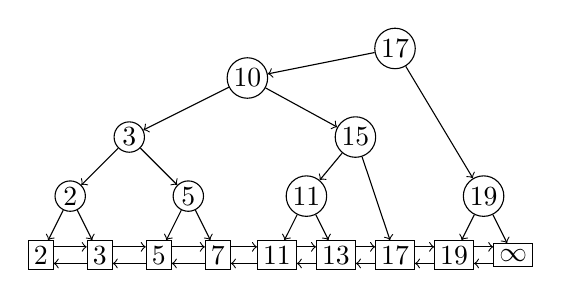
\begin{tikzpicture}[scale = .75]
    \begin{scope}[rectangle, every node/.style={draw}, inner sep = 2pt]
    \node (2) at (0,0) {2};
    \node (3) at (1,0) {3};
    \node (5) at (2,0) {5};
    \node (7) at (3,0) {7};
    \node (11) at (4,0) {11};
    \node (13) at (5,0) {13};
    \node (17) at (6,0) {17};
    \node (19) at (7,0) {19};
    \node (00) at (8,0) {$\infty$};
    \end{scope}
    \begin{scope}[circle, every node/.style={draw}, inner sep = 1pt]
    \node (2_) at (0.5, 1)  {2};
    \node (3_) at (1.5, 2)  {3};
    \node (5_) at (2.5, 1)  {5};
    \node (10_) at (3.5, 3)  {10};
    \node (11_) at (4.5, 1)  {11};
    \node (15_) at (5.33, 2)  {15};
    \node (17_) at (6, 3.5)  {17};
    \node (19_) at (7.5, 1)  {19};
    \end{scope}
    \begin{scope}[transform canvas = {yshift = 3pt}, ->]
      \draw  (2) -- (3);
      \draw  (3) -- (5);
      \draw  (5) -- (7);
      \draw  (7) -- (11);
      \draw  (11) -- (13);
      \draw  (13) -- (17);
      \draw  (17) -- (19);
      \draw  (19) -- (00);
    \end{scope}
    \begin{scope}[transform canvas = {yshift = -3pt}, <-]
      \draw (2) -- (3);
      \draw (3) -- (5);
      \draw (5) -- (7);
      \draw (7) -- (11);
      \draw (11) -- (13);
      \draw (13) -- (17);
      \draw (17) -- (19);
      \draw (19) -- (00);
    \end{scope}
    \begin{scope}[->]
      \draw (2_) -- (2);
      \draw (2_) -- (3);
      \draw (5_) -- (5);
      \draw (5_) -- (7);
      \draw (11_) -- (11);
      \draw (11_) -- (13);
      \draw (19_) -- (19);
      \draw (19_) -- (00);
      \draw (3_) -- (2_);
      \draw (3_) -- (5_);
      \draw (10_) -- (3_);
      \draw (10_) -- (15_);
      \draw (15_) -- (11_);
      \draw (15_) -- (17);
      \draw (17_) -- (10_);
      \draw (17_) -- (19_);
    \end{scope}
  \end{tikzpicture}
 \quad
 \begin{tikzpicture}[scale = .5]
   \begin{scope}
   \begin{scope}[circle, every node/.style={draw}, inner sep = 2pt]
     \node (x) at (1, 2) [label = above left:$v$] {};
     \node (y) at (0, 1)  [label = above left:$u$] {};
    \end{scope}
   \begin{scope}[every node/.style={
       	draw,isosceles triangle, 
	shape border rotate = 90},
     inner sep = 1pt]
    \node (A) at (-.75, -1)  {$A$};
    \node (B) at (.75, -1)  {$B$};
    \node (C) at (2, 0)  {$C$};
    \end{scope}
    \draw [->] (x)--(y);
    \draw [->] (x)--(C.apex);
    \draw [->] (y)--(A.apex);
    \draw [->] (y)--(B.apex);
   \end{scope}
   \begin{scope}[xshift = 6 cm]
   \begin{scope}[circle, every node/.style={draw}, inner sep = 2pt]
    \node (x) at (1, 1) [label = above right:$v$] {};
    \node (y) at (0, 2) [label = above right:$u$] {};
    \end{scope}
   \begin{scope}[every node/.style={
       	draw,isosceles triangle, 
	shape border rotate = 90},
     inner sep = 1pt]
    \node (A) at (-1, 0)  {$A$};
    \node (B) at (.25, -1)  {$B$};
    \node (C) at (1.75, -1)  {$C$};
    \end{scope}
    \draw [->] (y)--(x);
    \draw [->] (x)--(C.apex);
    \draw [->] (y)--(A.apex);
    \draw [->] (x)--(B.apex);
   \end{scope}
   \draw [thick, callout, ->] (2.5,2) to [bend left]  node [above, midway] {\emph{højredrejning}} (4.5,2);
   \draw [thick, callout, <-] (2.5,-1) to [bend right]  node [below, midway] {\emph{venstredrejning}} (4.5,-1) ;
 \end{tikzpicture}
\end{center}
\caption{\llabel{fig:bintree}\llabel{fig:rotate}\emph{Venstre}: Den sorterede følge $\seq{2,3,5,7,11,13,17,19}$, 
repræsenteret som et binært søgetræ.
\emph{Højre}: Drejning i et binært søgetræ.
  Trekanterne repræsenterer undertræer.
  Læg mærke til, at  knuderne $u$ og $v$ bytter forælder/barn-roller.
} 
\end{figure}


\begin{figure}
\begin{center}
\psfrag{e'}{$e'$}
\psfrag{e}{$e$}
\psfrag{k}{$k$}
\psfrag{u}{$u$}
\psfrag{T}{$T$}
\psfrag{v}{$v$}
\psfrag{insert e}{$\Id{tilføj}(e)$}
\includegraphics[scale=0.5]{img/insertnaive.eps}
\end{center}
\caption{\llabel{fig:insertnaive}Naiv indsættelse af indgang $e$ i et binært søgetræ. 
En trekant repræsenterer et helt undertræ.}
\end{figure}
\begin{figure}
\begin{center}
\psfrag{00}{$\infty$}
\psfrag{insert 17}{$\Id{tilføj}(17)$}
\psfrag{insert 13}{$\Id{tilføj}(13)$}
\psfrag{insert 11}{$\Id{tilføj}(11)$}
\psfrag{11}{$\!11$}
\psfrag{13}{$\!13$}
\psfrag{17}{$\!17$}
\psfrag{19}{$\!19$}
\includegraphics[width=\textwidth]{img/insertbin.eps}
\end{center}
\caption{\llabel{fig:insertbin}Naiv indsættelse af indgange i sorteret rækkefølge leder til, at træet degenererer til en liste.}
\end{figure}


\begin{exerc}
  Vis, at der for hvert mængde af $n\ge1$ indgange findes et binært søgetræ med $n+1$ blade og med dybde $\ceil{\log (n+1)}$.
\end{exerc}


Et søgetræ med $n+1$ blade og med dybde $\ceil{\log (n+1)}$ kaldes
\emph{perfekt balanceret}.
\index{sorteret følge!binært søgetræ!perfekt balanceret}
Det heraf resulterende logaritmiske søgetid udgør en dramatisk forbedring i forhold til den lineære søgetid $\Omega(n)$, som behøves for gennemløbning af en liste.
Den dårlige nyhed er, at det er ganske dyrt at opretholde den perfekt balance under indsættelse og fjernelse af indgange.
For at forstå problemet bedre, betragter vi den »naive« indsættelsesprocedure, som er vist i figur~\lref{fig:insertnaive}.
\index{sorteret følge!binært søgetræ!indsxt@\Id{indsæt}}
Vi lokaliserer den nye indgang $e$s nøgle $k$ i en liste, dvs. at vi finden den knude $e'$, som indeholder den på $k$ følgende nøgle.
Så tilføjes $e$ til listen, og en ny knude $v$ skabes med venstre barn $e$, højre barn $e'$ og spaltenøgle $k$.
Den tidligere forgænger til $e'$ peger nu på $v$.
I værste fald vælger hver indsættelse et blad på størst mulig dybde, sådan at træets dybde vokser hver gang.
Figur~\lref{fig:insertbin} viser et eksempel på denne effekt:
\index{sorteret følge!binært søgetræ!degenereret}: 
Træet kan degeneree til en liste, og vi er tilbage i en situation, som kræver lineær søgning.

En enkel løsning til dette problem er en sund portion optimisme:
Det værste fald behøver jo ikke at indtræffe.
Det viser sig faktisk, at indsættelsen af $n$ indgange i \emph{tilfældig} orden
\index{algoritmenanalyse!gennemsnits-}
fører til et træ, hvis gennemsnitlige dybde er omtrent $\approx 2.99\log n$ \cite{Dev86}.
\index{Devroye, L.}.
Vi skal her udelade beviset for denne påstand,
\index{sorteret følge!binært søgetræ!forventet dybde} 
men i stedet kort skitsere sammenhængen med kviksortering
\index{sortering!kviksortering}
for i det mindste at sandsynliggøre resultatet.
Hvordan kan man havne i et træ som i figur.~\lref{fig:bintree} ved naiv indsættelse?
Man begynder med at indsætte 17, dette opdeler mængden af indgange i delmængderne
$\{2,3,5,7,11,13\}$ og $\{19\}$.
Fra de resterende indgange i den første delmængde indsætter vi nu 7;
hvilket opdeler den i delmængderne $\{2,3,5\}$ og $\{11,13\}$.  
I terminologien fra kviksortering skulle vi sige, at 17 blev valgt som spalteførste rekursive kald, og 7 som næste kald for den venstre delmængde.
Opbygningen af et binært søgetræ og udførslen af kviksortering viser sig altså at være helt analoge processer, som udfører de samme sammenligninger, selvom det sker på forskellige tidspunkter.
Hver indgang sammenlignes med rodnøglen 17.
Ved kviksortering finder disse sammenligninger sted, når mængen opdeles i første kald i forhold til spaltenøglen 17.
Ved opbygningen af det binære søgetræ finder disse sammenligninger sted i forbindelse med indsættelsen af de enkelte indgange.
For eksempel sker sammenligningen mellem 17 og 11 under kviksortering i det første rekursive kald, mens det i søgetræet sker, når 11 bliver sat ind.
Vi har set i sætning~\ref{ch:sort:thm:cavg}, at kviksortering af $n$ indgange bruger forventet $O(n\log n)$ mange sammenligninger.
Ifølge den lige skitserede analogi er det forventede antal sammenligninger ved obbygningen af et binært søgetræ, hvor indgangene sættes ind i tilfældig rækkefølge, ligeledes $\O(n \log n)$. 
Derfor koster hver tilføjelse forventet $O(\log n)$ mange sammenligninger.
Man kan vise, at hver indsættelse behøver $O(\log n)$ mange sammenligninger med høj sandsynlighed, og at den gennemsnitlige dybde af træet er omtrent $2.99\log n$.   

Hvordan kan vi holde dybden logaritmisk i værste fald?
Der findes forskellige metoder, som sammenfattes i afsnit~\lref{s:further}, og hvoraf 2 betragtes nærmere i afsnit~\lref{s:abtree}. 
Først skal vi betragte in konstruktion, som tillader træknuder at have forskellig udgrad; derefter skal vi se, hvordan man kan holde binærtræer balancerede ved hjælp af rotationer.

\begin{exerc} 
  Figur~\lref{fig:rotate} viser, hvordan man kan ændre udseendet at et binærtræ med såkaldte rotationer. 
  \index{sorteret følge!binært søgetræ!rotation}
  Anvend gentagne rotationer på undetræerne i træet i figur~\lref{fig:rotate} for at gøre knuden med nøgle 11 til rodknude.
\end{exerc}

\begin{exerc}
  Forklar, hvordan man kan implementere et \emph{implicit}
  \index{sorteret følge!binært søgetræ!implicit} 
  binært søgetræ.
  Her er træet venstrefuldstændigt 
  \index{binærtræ!venstrefuldstændigt} og gemt som en række på samme måde som en binærhob (jf. afsnit~\ref{ch:pq:s:heap}).
  Hvad er fordele og ulemper sammenlignet med en pegerbaseret implementation?
  Sammenlign en søgeproces i det implicitte binærtræ med binærsøgning i en sorteret række.
\end{exerc}

%%%%%%%%%%%%%%%%%%%%%%%%%%%%%%%%%%%%%%%%%%%%%%%%%%%%%%%%%%%%%%%%%%%%%%
%\section{$(a,b)$-Bäume und Rot-Schwarz-Bäume}\llabel{s:abtree}%
\section{Ab-træer og rød-sorte træer}
\llabel{s:abtree}%
\index{sorteret følge!ab-træ|textbf}%
\index{ab-træ|sieheunter{sorteret følge}}%


%For positive heltal $a$ og $b$ med $a<b$ defineres et \emph{$a$-$b$-træ} som et søgetræ, hvori alle indre knuder bortset fra roden har (ud)grad mellem $a$ og $b$.
%Roden har grad 1 kun hvis træet har en enkelt blad.
%Ellers har roden grad mellem $2$ og $b$.
%Når $a\ge2$ og $b\geq 2a-1$, tillader fleksibiliten i udgraden, at vi kan sikre invarianten
%\index{invariant!datastruktur-}
%\index{sorteret følge!ab-træ@!invariant|textbf}
%at \emph{alle blade har samme dybde}.
%Betragt en knude med grad $d$.
%Til en sådan knude knytter vi en række $c[1..d]$ af børnepegere og en sorteret række $s[1..d-1]$ af $d-1$ spaltenøgler.
%Splitnøglern tjener til orientering under søgningen. 
%For at forenkle notationen definerer vi desuden $s[0]=-\infty$\ og $s[d]=\infty$. 
%Vi kræver for $i\in\{1,\ldots,d\}$, at nøglerne i indgangene i undertræet under det $i$te barn $c[i]$ ligger mellem den $(i-1)$te
%\index{sorteret følge!ab-Baum@$(a,b)$-Baum!Spaltschlüssel|textbf} 
%spaltenøgle (inklusive) og den $i$te spaltenøgle (ekslusive), mao., at der gælder $s[i-1] < \Id{nøgle}(e)\leq s[i]$.
%Figur~\lref{fig:prim} viser et 2-4-træ for følgen $\seq{2,3,5,7,11,13,17,19}$.
%
%
%%
%\begin{figure}[t]
%\begin{center}
%\psfrag{00}{{\footnotesize$\,\infty$}}
%\psfrag{r}{$r$}
%\psfrag{l}{$\ell$}
%\psfrag{height=2}{$\Id{height}=2$}
%\includegraphics[scale=0.4]{img/prim.eps}
%\end{center}
%\caption{\llabel{fig:prim}
%  Fremstilling af følgen $\seq{2,3,5,7,11,13,17,19}$ som et 2-4-træ. 
%  Træet har dybde ~$2$.}
%\end{figure}
%%
%\begin{figure}%
%\begin{tabbing}
%~~~~\=~~~~\=~~~~\=\kill
%\Class ABGreb $:$ \Pointer \To ABKnude \emph{eller} Knude\\
%\comment{En ABKnude [Item] er en knude i en navigationsdatastruktur}\\[3mm]
%\comment{En Knude er en knude i en dobbelthægtet liste.}\\[3mm]
%\Class ABKnude$(\Declare{\Id{spaltere}}{\Id{Følge} \Of \Id{Nøgle}},
%                \Declare{\Id{børn}}{\Id{Følge} \Of \Id{ABGreb}})$\+\\
%    \DeclareInit{$d$}{$1..b$}{$\abs{\Id{børn}}$}\comment{Grad}\\
%    \DeclareInit{$s$}{\Array$[1..b-1]$ \Of \Id{Nøgle}}{\Id{spaltere}}\\
%    \DeclareInit{$c$}{\Array$[1..b]$  \Of \Id{ABGreb}}{\Id{børn}}\\[2mm]
%    \Funct{lokaliserLokalt}{\Declare{$k$}{\Id{Nøgle}}}{$\NN$}\+\\
%      \Return $\min\{i\in 1..d\colon k\leq s[i]\}$\-\\[2mm]
%    \Funct{lokaliserRek}{\Declare{$k$}{\Id{Nøgle}}, \Declare{$h$}{$\NN$}}{\Id{ABGreb}}\+\\
%      $i$\,\Is\,lokaliserLokalt$(k)$\\      
%      \If $h=1$ \Then \+\\
%           \If $c[i]{\Points}e \ge k$ \Then \Return $c[i]$\\
%           \Else \Return $c[i]{\Points}\Id{next}$\-\\
%      \Else \Return $c[i]{\Points}$lokaliserRek$(k, 
%h-1)$\comment{\hspace*{1cm}\unitlength1in\begin{picture}(1.5,0)\put(-0.05,-0.05){\psfrag{i}{$i$}
% \psfrag{k=12}{$k=12$}\psfrag{h=1}{\hspace*{-2mm}$h=1$}\psfrag{h>1}{$h>1$}
% \includegraphics[width=1.5in]{img/locate.eps}}\end{picture}}\-\-\\[3mm]
%\Class ABTree$($\Declare{$a\geq 2$}{$\NN$}, \Declare{$b\geq 2a-1$}{$\NN$}$)$
%    \Of Element\+\\
%  \DeclareInit{$\ell$}{\Id{List} \Of \Id{Element}}{$\seq{\,}$}\\
%  \Declare{$r$}{ABKnude$(\seq{\,},\seq{\ell.\Id{head}})$}\\
%\DeclareInit{højde}{$\NN$}{$1$}\RRem{\hspace*{1cm}\unitlength1cm%
%\begin{picture}(2.5,0)\put(-0.05,-0.6){\psfrag{r}{$r$}\psfrag{l}{$\ell$}\psfrag{00}{$\infty$}%
%\includegraphics[width=0.8in]{img/empty.eps}}\end{picture}}\\[2mm]
%  \comment{Lokaliser indgangen med den mindste nøgle $k'\geq k$}\\
%  \Funct{lokaliser}{\Declare{$k$}{Nøgle}}{ABGreb}\+\\ 
%  \Return $r$.lokaliserRek$(k, \Id{højde})$
%\end{tabbing}
%
%\caption{
%  Ab-træer.
%  En (indre) knude
%  \index{sorteret følge!ab-træ!knude|textbf} 
%(\Id{ABKnude}) 
%  består af en følge af nøgler og en følge af greb for barneknuderne.
%  Graden er antallet af børn.
%  Vi stiller plads til rådighed til den maksimale grad $b$.
%  Til klassen \Id{ABKnude} hører to lokale funktioner (metoder):
%  $\Id{lokaliserLokalt}(k)$ finder bland følgen af spaltenøgler den rigtige plads for $k$;
%  proceduren $\Id{lokaliserRek}(k,h)$ går ud fra, at knuden \Id{ABKnude} har højde $h$, og klatrer yderligere $h$ niveauer ned i træet, for at finde det rigtige blad (\Id{Knude}) for $k$.
%  Konstruktøren for \Id{ABTræ} skaber et træ for den tomme følge, som består af et enkelt blad, nemlig attrapknuden med indgang $\infty$, samt en rod med grad 1. 
%  For at lokalisere nøglen $k$ i et ab-træ,
%  \index{sorteret følge!ab-træ!lokaliser@\emph{lokaliser}|textbf}
%  kaldes $r.\Id{lokaliserRek}(k,h)$, hvorved $r$ er roden og $h$ træets højde.}
%\end{figure}
%
%% TODO constant confusion of height and depth
%
%\begin{lemma}
%  \llabel{l:height} 
%  Dybden af et $a$-$b$-træ med $n\ge1$ indgange
%  \index{sorteret følge!ab-træ!dybde|textbf}
%  er højst
%\[ \displaystyle 1 + \floor{\log_a \frac{n+1}{2}} \,. \]
%\end{lemma}
%
%\begin{proof} 
%  Træet har $n+1$ blade, hvor termen  »$+1$« står for attrapbladet med nøgle $\infty$.
%
% For $n=0$ har toden grad 1, og der findes et enkelt blad.
% Betragt $n \ge 1$ og lad $h$ være træets dybde.
% Fordi rodgraden er mindst 2 og alle andre knuder har grad mindst $a$, er antallet af blade mindst $2 a^{h-1}$.
% Heraf følger $n+1 \ge 2 a^{h-1}$, dvs. $h \le 1 + \log_a ((n+1)/2)$.
% Nu følger grænsen, fordi dybden er et heltal.
%\end{proof}
%
%\begin{exerc}\llabel{ex:height}
%  Vis, at dybden af et $a$-$b$-træ med $n$ indgange er mindst $\ceil{\log_b (n+1)}$. 
%  Vis, at denne grænse samt grænsen fra lemma~\lref{l:height} er skarpe.
%\end{exerc}
%
%Søgning i et $a,b$-træ er ikke meget mere kompliceret end i et binært træ.
%Lad $k$ være søgenøglen og lad $k'$  være den mindste forekommende nøgle, som er mindst lige så stor som $k$.
%I en indre knude kan vi nu ikke længere nøjes med en enkelt sammenligning, fordi vi skal vælge det rigtige blandt op til $b$ børn.
%Med binær søgning i den sorterede følge af spaltenøgler kan det gøres med $\ceil{\log b}$ sammenligninger;
%denne omkostning opstår i hver knude på søgevejen.
%Søgemetodens korrekthed viser man med den samme invariant som bruges til søgning i et binært søgetræ:
%Det undertræ, som er rodfæstet ved den aktuelle knude, vil enten indeholde $k'$, eller i bladet længst til højre indeholde den umiddelbare listeforgænger til $k'$.
%Figur~\lref{alg:abtree} viser pseudokoden for opbygningen af  $a$-$b$-træer og operationen 
%\Id{lokaliser}.
%Idet vi bruger søgetræet til at navigere i en dobbelthægtet liste, som afsluttes af en attrapknude med nøgle  $\infty$, vil denne knude altid være bladet længst til højre i hele søgetræet.
%Derfor kan roden ikke have grad $0$, og en søgning efter en nøgle, som er større end alle egentlige nøgler i listen, returnerer et greb på attrapknuden.
%
%\begin{exerc} 
%  Vis, at det samlede antal sammenligninger ved søgning i et $a$-$b$-træ er højst 
%  $\lceil\log b\rceil\cdot (1 + \log_a ((n+1)/2))$.
%  Vis, at dette  er  $O(\log b) + O(\log n)$ for $b \le 2a$.
%  Hvad er konstanten foran $(\log n)$-termen?
%\end{exerc}
%
%\begin{figure}[b]
%\begin{center}
%\psfrag{c1}{$c_1$}\psfrag{c2}{$c_2$}\psfrag{c3}{$c_3$}\psfrag{c4}{$c_4$}\psfrag{c5}{$c_5$}
%\psfrag{u}{$u$}\psfrag{v}{$v$}\psfrag{t}{$t$}\psfrag{k}{$k$}
%%\includegraphics[width=]{img/addleafandsplit2,width=0.6\textwidth}
%\includegraphics[scale=0.5]{img/addleafandsplit2}
%\end{center}
%\caption{Knudekløvning:
%Knuden $v$ med grad $b+1$ (her: 5) kløves i to knuder med grad $\floor{(b+1)/2}$ henholdsvis $\ceil{(b+1)/2}$.
%Forgængerknuden øges med $1$.
%Spaltenøglen, som deler $v$ to »dele«, flyttes til forgængerknuden.
%\llabel{fig:addleafandsplit}}
%\end{figure}
%
%
%For at \emph{tilføje} 
%\index{sorteret følge!ab-træ@$a$-$b$-træ!tilføje@\Id{tilføj}|textbf} 
%en indgang $e$ med nøgle $k=\Id{nøgle}(e)$ klatrer vi først rekursivt nedad i træet, for at lokalisere nøglen $k$ i listen.
%% TODO klatrer vi i træer? vandrer vi? 
%Herved finder vi en listeindgang $e'$.
%Nu er $e'$ enten den ingang med mindst nøgle, som er mindst lige så stor som $k$, eller den umiddelbare listeforgænger til denne indgang.
%(Det sidstnævnte kan kun indtræffe, hvis $k$ ikke forekommer i listen.)
%Først undersøger vi, om  $k=\Id{nøgle}(e')$, i hvilket fald vi blot erstatter indgangen $e'$ med $e$.
%Dette sikrer også, at ingen nøgle forekommer to gange i følgen.
%Hvis $k < \Id{nøgle}(e')$, skal en ny listeknude med indgang $e$ føjes ind umiddelbart før $e'$. 
%For at undgå at behandle tilfældet $k > \Id{nøgle}(e')$ separat, reducerer vi til det første tilfælde.
%Hertil skaber vi en ny listeknude med indgang $e$ og bytter den rundt med $e'$
%både i den dobbelthægtede liste og med hensyn til barnepegeren fra naviationsdatastrukturen.
%%
%\begin{buchalgorithmpos}{htbp}{alg:abinsert}{Indsættelse i et $a$--$b$-træ.}%
%\Rem{Eksempel:\hspace*{8cm}\unitlength1cm\begin{picture}(7,2)\put(-4,-3){\psfrag{00}{{\small\hspace*{0.5mm}$\infty$}}\psfrag{r}{{\footnotesize$r$}}\psfrag{k=3, t=}{{\footnotesize$k{=}3{,}t{=}$}}\includegraphics[scale=0.34]{img/insertexall.eps}}\end{picture}}\\
%\Rem{$\seq{2,3,5}.\Id{tilføj}(12)$}\\
%  \Procedure ABTræ\emph{::}\Id{indsæt}(\Declare{$e$}{Element})\+\\ 
%  $(k,t)\Is r.\Id{indsætRek}(e, \Id{højde}, \ell)$\\
%  \If $t\neq\Null$ \Then \quad \RRem{Roden blev kløvet\hspace*{7cm}}\+\\ 
%    $r\Is \Allocate \Id{ABKnude}(\seq{k}, \seq{t, r})$\\
%    height\Increment\-\-\\[2mm]
%%
%\Rem{Indføj en ny indgang i et undertræ af dybde $h$.}\\
%  \Rem{Hvis dette kløver undertræets rod,}\\ 
%\Rem{returneres en ny spaltenøgle og et greb til det nye undertræ.}\\
%\Funct{ABKnude\emph{::}indsætRek}{\Declare{$e$}{\Id{Element}}, \Declare{$h$}{$\NN$}, \Declare{$\ell$}{Liste \Of Element}}{Nøgle$\times$ABGreb}\+\\
%  $i\Is \Id{lokaliserLokalt}(e)$\\      
%  \If $h=1$ \Then\+\quad\Rem{Basis, nederste træniveau}\\
%    \If $\Id{nøgle}(c[i]{\Points} e)=\Id{nøgle}(e)$ \Then\+\\
%      $c[i]{\Points} e\Is e$\\
%      \Return$(\bot,\Null)$\-\\
%    \Else\+\\ 
%    \If $\Id{nøgle}(c[i]{\Points}e)>\Id{nøgle}(e)$ \Then\+\\
%     $(k,t)\Is (\Id{nøgle}(e), \ell.\Id{indsætFør}(e,c[i]))$\RRem{\unitlength1in\begin{picture}(1.1,0)\put(-0,-0.1){\psfrag{00}{{\small\hspace*{0.5mm}$\infty$}}\psfrag{t}{{\footnotesize$t$}}\psfrag{c[i]}{{\footnotesize$c[i]$}}\includegraphics[scale=0.34]{img/insertlist.eps}}\end{picture}}\-\\
%    \Else \+\quad  \Rem{$\Id{nøgle}(c[i]{\Points}e)<\Id{nøgle}(e)$}                     \\
%      $(k,t)\Is (\Id{nøgle}(c[i]{\Points} e), \ell.\Id{indsætEfter}(e,c[i]))$\\
%      \Id{ombyt}$(c[i],t)$\-\-\\
%  \Endif\-\\
%      \Else\+\\ 
%    $(k,t)\Is c[i]{\Points}\Id{indsætRek}(e, h-1, \ell)$\\
%    \If $t=\Null$ \Then \Return $(\bot,\Null)$\-\\
%  \Endif\\[2.5mm]
%  $s'\Is \seq{s[1],\ldots, s[i-1], k  ,s[i],\ldots,s[d-1]}$\\
%  $c'\Is \seq{c[1],\ldots, c[i-1], t  ,c[i],\ldots,c[d]}$\RRem{\unitlength1in\begin{picture}(1.3,0)\put(0,-0.1){\psfrag{00}{{\small\hspace*{0.5mm}$\infty$}}\psfrag{t}{{\footnotesize$t$}}\psfrag{s'}{{\footnotesize$s'$}}\psfrag{c'}{{\footnotesize$c'$}}\psfrag{12=k}{{\footnotesize$12=k$}}\includegraphics[scale=0.36]{img/insert1b.eps}}\end{picture}}\\[2.5mm]
%  \If $d< b$ \Then\+\quad\Rem{der er stadig plads i knuden}\\
%    $(s,c,d)\Is (s',c',d+1)$\\
%    \Return $(\bot,\Null)$\-\\
%  \Else\+\quad\Rem{kløv denne knude}\\
%    $d\Is \floor{(b+1)/2}$\\
%    $s\Is s'[b+2-d..b]$\\
%    $c\Is c'[b+2-d..b+1]$\RRem{\unitlength1in\psfrag{00}{{\small\hspace*{0.5mm}$\infty$}}\psfrag{s}{{\footnotesize$s$}}\psfrag{c}{{\footnotesize$c$}}\begin{picture}(1.3,0)\put(0,0){\includegraphics[scale=0.36]{img/insert2b.eps}}\end{picture}}\\
%    \Return $(s'[b+1-d],\Allocate ABKnude(s'[1..b-d], 
%                                    c'[1..b+1-d]))$
%\end{buchalgorithmpos}%
%%
%Metoden for lokalisering ved indsættelse sikrer, at en søgning efter $\Id{nøgle}(e')$ ville føre til knuden med indgang $e$. 
%Vi kan altså præcis som i det første tilfælde indsætte
% $e'$-listeknuden umiddelbart  før $e$-listeknuden. 
%Fra nu af koncentrerer vi os på det tilfælde, hvor $e$-knuden bliver indsat før $e'$-knuden i listen $\ell$.
%Hvis $e'$-knuden er det  $i$te barn $c[i]$ af sin forgængerknude $v$, så bliver $e$-knuden nu gjort til det nye barn $c[i]$, og værdien $k$ givet ved $k=\Id{nøgle}(e)$ er den nye spaltenøgle $s[i]$.
%De tidligere børn $c[i..d]$ og deres spaltenøgler $s[i..d-1]$ flyttes til højre med en indeksposition.
%Hvis $d$ var mindre end $b$, kan $d$ nu øges med 1, og indsættelsen er færdig.
% 
%Det vanskelige tilfælde opstår, når $v$ allerede havde grad $d=b$ og nu ville få grad $b+1$.
%Lad $s'$ værre rækken af spaltenøgler i denne overfulde knude, lad $c'$ være rækken af børnepegere, og lad $u$ være forgængeren til $v$ (hvis den eksisterer).
%Vi løser problemet ved \emph{flække} knuden $v$ midtover
%som vist i figur \lref{fig:addleafandsplit}). 
%\index{sorteret følge!ab-træ@$a$-$b$-træ!\Id{flæk} (knude)|textbf}
%Nærmere betegnet skaber vi en ny knude $t$ og sænker $v$s grad $d$ til  $\ceil{(b+1)/2}$ ved at flytte de $b+1-d$ første børnepegere $c'[1..(b+1-d)]$ og de tilsvarende nøgler$s'[1..(b-d)]$ fra $v$ til den nye knude $t$.
%Den gamle knude $v$ beholder de $d$ børnepegere $c'[(b+2-d)..(b+1)]$ længst til højre og de tilsvarende spaltenøgler $s'[(b+2-d)..b]$, men flytter disse værdier til venstre i deres rækker med henholdsvis $d$ og $d-1$ positioner. 
%
%Hvor gør vi af den »overflødige« midterste spaltenøgle $k$ med værdi $k=s'[b+1-d]$? 
%Fordi værdien af $k$ er en øvre grænse for alle nøgler i undertræet med rod $t$, skal den bruges i $v$s forgænger $u$, sammen med en peger på $t$.
%Situationen i $u$ modsvarer præcis situationen i $u$ inden indsættelsen:
%fordi $v$ før var det $i$te barn af $u$, skal $t$ nu indtage denne plads; de andre børn til $u$ fra og med position $i$ rykker en position til højre.
%Tilsvarende indtager $k$ rollen som den $i$te spaltenøgle. 
%Disse ændringer i $u$ øger dens grad med $1$.
%Skulle graden blive lig med $b+1$, flækkes $u$.
%Denne proces fortsætter, til nogen forgænger $v$ har plads til et nyt barn, eller til rodknuden selv bliver flækket.
%
%\emph{TODO: resten udeladt}

%I det sidste tilfælde skaber vi en ny rodknude, so peger på den gamle rodknudes to halvdele.
%Dette er den eneste situation, i hvilken træets dybde kan vokse.
%Når det sker, forøges dybden af samtlige blade med $1$.
%Invarianten TODO
%In diesem Fall nimmt die Tiefe aller Blätter um 1 zu, d.\,h.,  
%die Invariante, dass alle Blätter auf demselben Level sitzen, 
%bleibt erhalten. 
%Weil nach Lemma~\lref{l:height} die Tiefe des Baums $\Oh{\log n}$ ist, 
%%and since \Id{tilføj} performs at most
%%$\Oh{1}$ operations in a node,
%ergibt sich für \Id{tilføj} eine Ausführungszeit von
%$\Oh{\log n}$ im schlechtesten Fall. Pseudocode für die Einfügung
%findet man in 
%Abb.~\lref{alg:abinsert}.\footnote{Die Schreibweise \Id{C}::\Id{m} ist aus \CC\ 
%übernommen, um die Definition einer Methode \Id{m} für eine Klasse \Id{C} zu bezeichnen.}
%
%
%Wir müssen noch begründen, weshalb $\Id{tilføj}$ einen korrekten
%$(a,b)$-Baum erzeugt. Wenn ein Knoten mit Grad $b+1$ gespaltet wird, 
%entstehen Knoten mit Grad
%$d=\ceil{(b+1)/2}$ und $b+1-d$. Diese Grade sind offensichtlich kleiner als $b$. 
%Weiter folgt aus der Ungleichung $b \ge 2a - 1$, dass  
%$b +1 - \ceil{(b+1)/2}\geq a$ gilt. 
%Man mache sich klar, dass $b = 2a-2$ ungeeignet ist. 
%
%
%%
%\begin{exerc}
%Man ist versucht, die Prozedur \Id{tilføj} kompakter zu programmieren,
%indem man \Id{lokaliser} aufruft, um den anfänglichen Abstieg im Baum zu organisieren. 
%Warum funktioniert das nicht?
%Könnte man so vorgehen, wenn jeder Knoten einen Zeiger zu seinem Vorgänger hätte?
%\end{exerc}
%%
%%
%\begin{buchalgorithmpos}{t}{alg:abremove}{Löschen in einem $(a,b)$-Baum.}\quad\\
%\hspace*{-2pt}\Rem{Beispiel: $\seq{2,3,5}$.remove$(5)$}\\
%\Procedure ABTree\emph{::}remove$(\Declare{k}{\Id{Key}})$\+\RRem{\unitlength1in\begin{picture}(1.1,0)\put(0,-0.58){\psfrag{00}{{\small\hspace*{0.5mm}$\infty$}}\psfrag{r}{{\footnotesize$r$}}\psfrag{k}{{\footnotesize$k$}}\includegraphics[scale=0.34]{img/del1.eps}}\end{picture}}\hspace*{1.5in}\\ 
%%  \Assert $\exists e\in\ell\gilt \Id{nøgle}(e)=k$\\
%  $r$.removeRec$(k, \Id{height}, \ell)$\\
%  \If $r.d=1\wedge \Id{height}>1$ \Then\+\\ 
%    $r'\Is r$\emph{;} $r\Is r'.c[1]$\emph{;}\\ 
%		\Delete $r'$\emph{;} $\Id{height}\Decrement$
%\RRem{\unitlength1in\begin{picture}(0.9,-0)\put(-0.0,-0.08){\psfrag{00}{{\small$\infty$}}\psfrag{r}{{\footnotesize$r$}}\psfrag{k}{{\footnotesize$k$}}\includegraphics[scale=0.34]{img/del4.eps}}\end{picture}}\-\-\\[4mm]
%%
%\Procedure ABKnude\emph{::}removeRec$(\Declare{k}{Key}, \Declare{h}{\NN}, \Declare{\ell}{\text{List \Of Element}})$\+\\
%  $i\Is \Id{locateLocally}(k)$\\
%  \If $h=1$ \Then\+\quad\Rem{Basisfall, unterstes Baumlevel}\\ 
%    \If $\Id{nøgle}(c[i]{\Points} e)=k$ \Then\quad\Rem{es gibt etwas zu löschen}\+\\
%    $\ell.\Id{fjern}(c[i])$\\
%    removeLocally$(i)$\RRem{\unitlength1in\begin{picture}(1.2,-0)\put(0,-0.2){\psfrag{00}{{\small$\infty$}}\psfrag{r}{{\footnotesize$r$}}\psfrag{s}{{\footnotesize$s$}}\psfrag{c}{{\footnotesize$c$}}\psfrag{i}{{\footnotesize$i$}}\includegraphics[scale=0.34]{img/del2.eps}}\end{picture}}\-\-\\
%  \Else\+\\
%    $c[i]{\Points} \Id{removeRec}(e, h-1, \ell)$\\
%    \If $c[i]{\Points} d < a$ \Then\+\RRem{Invariante muss repariert werden}\\
%      \If $i=d$ \Then $i\Decrement$\RRem{$i$ und $i+1$ müssen gültige Indizes sein}\\
%%MD Original, eine Klammer zu viel:      $s'\Is \Id{concatenate}(c[i]{\Points} s, \seq{s[i]}, c[i+1]{\Points} s))$ Korrekt: \\
%                $s'\Is \Id{concatenate}(c[i]{\Points} s, \seq{s[i]}, c[i+1]{\Points} s)$\\
%       $c'\Is \Id{concatenate}(c[i]{\Points} c, c[i+1]{\Points} c)$\\
%      $d'\Is \abs{c'}$\\
%    \If $d'\leq b$ \Then\quad\Rem{verschmelzen: "`\hspace*{1.5pt}\Id{fuse}"'}\+\\
%      $(c[i+1]{\Points} s, c[i+1]{\Points} c, c[i+1]{\Points} d)\Is (s', c', d')$\\
%      \Dispose $c[i]$\emph{;}\quad removeLocally$(i)$\RRem{\unitlength1in\begin{picture}(1,-0)\put(0.1,-0.3){\psfrag{00}{{\small$\infty$}}\psfrag{r}{{\footnotesize$r$}}\psfrag{s}{{\footnotesize$s$}}\psfrag{c}{{\footnotesize$c$}}\psfrag{s'}{{\footnotesize$s'$}}\psfrag{c'}{{\footnotesize$c'$}}\psfrag{i}{{\footnotesize$i$}}\includegraphics[scale=0.34]{img/del3.eps}}\end{picture}}\-\\
%    \Else\+\>\>\>\>\Rem{ausbalancieren: "`\hspace*{1pt}\Id{balance}"'}\\
%      $m\Is \ceil{d'/2}$\\
%      $(c[i]{\Points} s, c[i]{\Points} c, c[i]{\Points} d)\Is (s'[1..m-1], c'[1..m], m)$\\
%      $(c[i+1]{\Points} s,$\>\>\>\>\>\>\> $c[i+1]{\Points} c,$\quad $c[i+1]{\Points} d)\,\,\Is$\+\\ 
%      $(s'[m+1..d'-1],$\>\>\>\>\>\>$c'[m+1..d'],$\quad $d'-m)$\-\\
%      $s[i]\Is s'[m]$\-\-\-\-\\[2mm]
%%      
%\Rem{Lösche das $i$-te Kind eines Baumknotens}\\
%\Procedure ABKnude\emph{::}removeLocally$(\Declare{i}{\NN})$\+\\
%  $c[i..d-1]\Is c[i+1..d]$\\
%  $s[i..d-2]\Is s[i+1..d-1]$\RRem{\unitlength1in\begin{picture}(1.5,-0)\put(0,-0.0){\psfrag{i}{{\footnotesize$i$}}\psfrag{k1}{{\footnotesize$k_1$}}\psfrag{k2}{{\footnotesize$k_2$}}\psfrag{k3}{{\footnotesize$k_3$}}\psfrag{A}{{\scriptsize$T_1$}}\psfrag{B}{{\scriptsize$T_2$}}\psfrag{C}{{\scriptsize$T_3$}}\psfrag{D}{{\scriptsize$T_4$}}\psfrag{cc}{{\footnotesize$c$}}\psfrag{s}{{\footnotesize$s$}}\includegraphics[scale=0.4]{img/del5.eps}}\end{picture}}\\
%  $d$\Decrement
%\end{buchalgorithmpos}%
%%
%%
%\begin{figure}[t]
%\begin{center}
%\psfrag{c1}{$c_1$}\psfrag{c2}{$c_2$}\psfrag{c3}{$c_3$}\psfrag{c4}{$c_4$}\psfrag{c5}{$c_5$}
%\psfrag{u}{$u$}\psfrag{v}{$v$}\psfrag{t}{$t$}\psfrag{k1}{$k_1$}\psfrag{k2}{$k_2$}\psfrag{k}{$k$}
%%\includegraphics[width=]{img/fusingandbalancing2,width=0.9\textwidth}
%\includegraphics[scale=0.5]{img/fusingandbalancing2}
%\end{center}
%\caption{\llabel{fig:balanceandfuse} Knotenbalancierung ("`\Id{balance}"') und Verschmelzen ("`\Id{fuse}"') bei (2,4)-Bäumen: Knoten $v$ hat
%Grad $a-1$ (hier: 1). \emph{Links}: Knoten $v$ hat einen Geschwisterknoten mit Grad
%$a+1$ oder mehr (hier: 3), und wir \emph{balancieren} die Grade \emph{aus}. 
%\emph{Rechts}: Der Geschwisterknoten hat Grad $a$, und wir \emph{verschmelzen} $v$ 
%mit diesem Geschwisterknoten. 
%Man beobachte, wie die Spaltschlüssel verschoben werden.
%Wenn zwei Knoten verschmolzen werden, verringert sich der Grad des Vorgängers um 1.}
%\end{figure}
%%
%%
%Wir wenden uns nun der Löschoperation \Id{fjern}\index{sorteret følge!ab-Baum@$(a,b)$-Baum!remove@\Id{fjern}|textbf}
%für $(a,b)$-Bäume zu.
%Der Ansatz ist ähnlich wie bei \Id{tilføj}. 
%Wir lokalisieren den zu löschenden Eintrag, 
%entfernen seinen Knoten aus der doppelt verketteten Liste
%und reparieren mögliche Verletzungen der Invarianten auf dem Rückweg nach oben. 
%In Abb.~\lref{alg:abremove} ist Pseudocode für diese Operation angegeben. 
%Wenn einem Knoten $u$ als Resultat einer Löschung im 
%Unterbaum unter Kindknoten $c[i]$ mitgeteilt wird, dass der Grad von $c[i]$  
%auf $a-1$ gefallen ist, dann wird, von $u$ ausgehend, dieser Kindknoten mit
%einem seiner Geschwister $c[i-1]$ oder $c[i+1]$ kombiniert, 
%um die Invariante wiederherzustellen. 
%Dabei gibt es zwei Fälle, die in Abb.~\lref{fig:balanceandfuse} bildlich dargestellt sind. 
%Wenn der Grad des Geschwisterknotens größer als $a$ ist, können wir 
%die Grade \emph{ausbalancieren}\index{sorteret følge!ab-Baum@$(a,b)$-Baum!ausbalancieren|textbf},
%indem wir einen oder mehrere Kinder des Geschwisterknotens nach $c[i]$ schieben.
%Wenn der Geschwisterknoten aber Grad exakt $a$ hat, nützt Ausbalancieren nichts, 
%weil beide Knoten zusammen nur $2a-1$ Kinder haben, so dass 
%es unmöglich ist, beiden $a$ Kinder zu geben.  
%Wir können aber die beiden Knoten zu einem \emph{verschmelzen}\index{sorteret følge!ab-Baum@$(a,b)$-Baum!verschmelzen|textbf},
%weil die Regel $b\geq 2a-1$ sicherstellt, 
%dass der Grad des durch die Verschmelzung entstandenen Knotens 
%nicht größer als $b$ ist. 
%%
%
%Um den Knoten $c[i]$ mit seinem rechten Geschwister $c[i+1]$ zu verschmelzen, 
%konkatenieren wir die Kindarrays der beiden Knoten und speichern das Ergebnis in
%Knoten $c[i+1]$.  
%Die Spaltschlüssel können ebenfalls (in das entsprechende Array in  $c[i+1]$) übernommen werden,
%mit Ausnahme der Stelle, an der die beiden Folgen zusammengefügt werden:
%hier wird der Spaltschlüssel $s[i]$ des Vorgängerknotens $u$ eingetragen.
%Nun kann man den Knoten $c[i]$ freigeben,
%und die Position $c[i]$ sowie den Spaltschlüssel $s[i]$
%aus den entsprechenden Arrays im Vorgängerknoten $u$ streichen.
%(Hierdurch rückt der Griff für den neuen Knoten auf Position $c[i]$ vor.) 
%
%
%\begin{exerc}
%Nehmen Sie an, dass ein Knoten $v$ 
%durch eine Verschmelzung wie eben beschrieben entstanden ist. 
%Zeigen Sie, dass die Ordnungsinvariante erhalten bleibt:
%Ein Eintrag $e$, der über Kind $v.c[i]$ erreichbar ist, 
%erfüllt $v.s[i-1]<\Id{nøgle}(e)\leq v.s[i]$, für $1\leq i\leq v.d$.
%\end{exerc}
%
%
%Das Ausbalancieren von zwei benachbarten Geschwistern
%ist äquivalent dazu, sie erst zu verschmelzen und dann
%das Ergebnis zu spalten, wie in der Operation \Id{tilføj}. 
%Weil das Verschmelzen von zwei Knoten den Grad 
%ihres Vorgängers verringert,
%kann sich die Notwendigkeit, Knoten auszubalancieren oder zu verschmelzen, 
%durch den Baum von unten nach oben fortpflanzen. 
%Wenn irgendwann einmal der Grad der Wurzel auf 1 fällt,
%gibt es zwei Möglichkeiten. 
%Wenn der Baum Tiefe 1 hat, 
%die Liste also nur einen Eintrag hat (den Dummyeintrag mit Schlüssel $\infty$),
%dann ist nichts weiter zu tun. 
%Andernfalls können wir den Wurzelknoten freigeben und 
%das einzige Kind als neue Wurzel benützen. 
%Die Höhe des Baums verringert sich dabei um 1. 
%
%
%Die Ausführungszeit von \Id{fjern} 
%ist ebenfalls proportional zur Höhe des Baums und daher logarithmisch in 
%der Größe der sortierten Folge. 
%Wir fassen das Rechenzeitverhalten von $(a,b)$-Bäumen im folgenden Satz zusammen.
%%
%\begin{satz}
%Für ganze Zahlen $a$ und $b$ mit $a \ge 2$ und $b\geq 2a-1$ gilt:
%$(a,b)$-Bäume führen die Operationen \Id{tilføj}, \Id{fjern} und \Id{lokaliser}
%auf sortierten Folgen mit $n$ Einträgen in Zeit $\Oh{\log n}$ aus. 
%\end{satz}
%%
%
%\begin{exerc}\llabel{ex:local}
%Geben Sie eine detailliertere Implementierung von \Id{locateLocally}
%an, die auf binärer Suche beruht und nicht mehr als $\ceil{\log b}$ 
%Vergleiche benötigt. 
%Dabei sollten Sie es vermeiden, explizit unendliche Schlüsselwerte zu benutzen, 
%und es sollte keine Fallunterscheidungen für Grenzfälle geben. 
%% l=0
%% r=d
%% m=d div 2
%% invariant s[l] < k <= s[r]
%% loop
%%   if s[m] < k then 
%%     l = m
%%   else // k <= s[m]            
%%     r = m
%%   if l+1 = r then return r
%%   m = (l + r) div 2
%%% use switch(d){...} for fast (2,4)-trees
%\end{exerc}
%
%\begin{exerc}\llabel{ex:compares}
%Nehmen Sie $a=2^k$ und $b=2a$ an. Zeigen Sie, dass für eine \Id{lokaliser}-Operation
%in einem $(a,b)$-Baum mit $n$ Einträgen $(1+\frac{1}{k})\log n+1$
%Schlüsselvergleiche ausreichen. 
%\emph{Hinweis}: Es genügt \emph{nicht} ganz, Aufgabe~\lref{ex:height}
%mit Aufgabe~\lref{ex:local} zu kombinieren, da dies einen 
%zusätzlichen Summanden $+\,k$ erzeugen würde.
%\end{exerc}%
%%
%%
%\begin{exerc}\llabel{ex:multiple keys} 
%Erweitern Sie $(a,b)$-Bäume so, dass sie mit mehrfach vorkommenden Schlüsseln 
%umgehen können. 
%Einträge mit identischen Schlüsseln sollen dabei in \emph{last-in-first-out}-Manier
%behandelt werden, d.\,h., $\Id{fjern}(k)$ soll den Eintrag mit Schlüssel $k$
%entfernen, der als letzter eingefügt wurde.
%\end{exerc}%
%%
%\begin{figure}[t]
%\begin{center}\psfrag{or}{or}
%\includegraphics[width=\textwidth]{img/twofourredblack2}
%\end{center}
%\caption{\llabel{fig:correspondance red--black and (2,4)} 
%(2,4)-Bäume und Rot-Schwarz-Bäume entsprechen einander. 
%Knoten mit Grad 2, 3 bzw. 4  (jeweils \emph{links})
%entsprechen den jeweils \emph{rechts} angegebenen Konfigurationen. 
%Rote Kanten sind {\bf fett} gezeichnet.}
%\end{figure}%
%%
%\end{figure}%
%}%
%%
%%
%\begin{exercisestara}[Rot-Schwarz-Bäume]\index{sorteret følge!Rot-Schwarz-Baum}\index{Rot-Schwarz-Baum|sieheunter{sorteret følge}}
%Ein \emph{Rot-Schwarz-Baum} ist ein binärer Suchbaum,
%in dem jede Kante rot oder schwarz \emph{gefärbt} ist, so dass
%die folgenden Invarianten gelten. 
%Die \emph{Schwarz-Tiefe} eines Knotens $v$ ist dabei die Anzahl der schwarzen Kanten
%auf dem Weg von der Wurzel zu $v$.
%\begin{enumerate}
%\item[(a)] Alle Blätter haben die gleiche Schwarz-Tiefe.
%\item[(b)] Eingangskanten von Blättern sind schwarz. 
%\item[(c)] Kein Weg von einer Wurzel zu einem Blatt enthält zwei aufeinanderfolgende rote Kanten. 
%\end{enumerate}
%Zeigen Sie, dass Rot-Schwarz-Bäume und $(2,4)$-Bäume in folgendem Sinn isomorph sind:
%Aus einem $(2,4)$-Baum kann man einen Rot-Schwarz-Baum gewinnen, 
%indem man Knoten von Grad 3 bzw. 4 durch 2 bzw. 3 Knoten ersetzt,
%die untereinander durch rote Kanten verbunden sind, wie in 
%Abb.~\lref{fig:correspondance red--black and (2,4)} skizziert. 
%Aus einem Rot-Schwarz-Baum kann man mit der inversen Transformation einen $(2,4)$-Baum gewinnen,
%indem man Komponenten, die durch rote Kanten verbunden sind, durch einen einzigen
%Knoten mit Grad 3 oder 4 ersetzt. 
%Erklären Sie, wie man $(2,4)$-Bäume implementieren kann, 
%indem man sie als Rot-Schwarz-Bäume darstellt.%   
%\footnote{Falls die Schlüssel großen Umfang haben, 
%könnte dies platzeffizienter sein als eine direkte Darstellung.}
%Erklären Sie insbesondere, wie die bei $(2,4)$-Bäumen auftretenden
%Operationen der Vergrößerung und Verringerung des Grades eines Knotens,
%das Spalten und Verschmelzen von Knoten, und die Rebalancierung
%mit Hilfe von Rotationsoperationen\index{sorteret følge!binärer Suchbaum!Rotation} 
%(s. Abb.~\lref{fig:rotate}) und Umfärbungen im Rot-Schwarz-Baum 
%nachgebaut werden können. Die Farben sind jeweils in den Zielknoten der 
%entsprechenden Kanten gespeichert.
%\end{exercisestara}
%
%
%
%%%%%%%%%%%%%%%%%%%%%%%%%%%%%%%%%%%%%%%%%%%%%%%%%%%%%%%%%%%%%%%%%%%%%%%
%\section{Weitere Operationen}\llabel{s:operations}
%
%
%
%Mit Suchbäumen lassen sich über \Id{tilføj}, \Id{fjern} und \Id{lokaliser} hinaus 
%noch viele andere Operationen auf sortierten Listen
%realisieren.
%Wir werden solche Operationen in zwei Gruppen betrachten:
%In diesem Abschnitt geht es um Operationen, die sich 
%direkt mit $(a,b)$-Bäumen ausführen lassen,
%in Abschnitt~\lref{s:augment} werden wir Operationen 
%betrachten, für die man die Datenstruktur erweitern muss.    
%
%
%\begin{itemize}
%\item \emph{min/max}.
%Die Operationen \Id{første}\index{sorteret følge!first@\Id{første}}\index{Liste!first@\Id{første}} 
%und \Id{sidste}\index{Liste!last@\Id{sidste}}\index{sorteret følge!last@\Id{sidste}},
%die für sortierte Listen zur Verfügung stehen, liefern in konstanter Zeit den kleinsten und
%den größten Eintrag der sortierten Folge.
%Beispielsweise finden wir in Abb.~\lref{fig:prim}
%über den Dummyknoten mit dem Schlüssel $\infty$ mit Hilfe der \Id{next}- und \Id{prev}-Zeiger
%sofort den kleinsten Schlüssel, $2$, und den größten Schlüssel, $19$.
%Insbesondere implementieren sorteret følgen \emph{zweiseitige Prioritätswarteschlangen}
%(engl.: \emph{double-ended priority queues})\index{Prioritätswarteschlange!zweiseitige},
%d.\,h., Mengen, bei denen man den kleinsten oder den größten
%Eintrag finden und entnehmen kann,
%wobei Suchen in konstanter Zeit und Entnehmen in logarithmischer Zeit ausgeführt werden kann.
%
%\item \emph{Bereichsanfragen} (engl.: \emph{range queries}).\index{sorteret følge!Bereichssuche} 
%  Um alle Einträge mit Schlüsseln im Intervall ("`Bereich"') $[x,y]$ zu finden und auszugeben, 
%  lokalisieren wir $x$ und durchlaufen dann die sortierte Liste, 
%  bis wir einen Eintrag mit einem Schlüssel erreichen, der größer als $y$ ist. 
%  Die hierfür benötigte Zeit ist $\mathrm{O}\!(\log n + {}$Umfang der Aus\-gabe{}$)$.
%  Beispielsweise wird die Bereichsanfrage $[4,14]$ im Suchbaum in Abb.~\lref{fig:prim} 
%  zunächst den Eintrag $5$ finden, danach 
%  $7$, $11$ und  $13$ ausgeben, und beim Erreichen der $17$ anhalten.
%
%\item \emph{(Neu-)Aufbau.}\index{sorteret følge!ab-Baum@$(a,b)$-Baum!Aufbau@(Neu-)Aufbau|textbf} 
%In Aufgabe~\lref{ex:rebuild} werden Sie gebeten, einen Algorithmus anzugeben, 
%der in Linearzeit aus einer sortierten Liste oder einem sortierten Array 
%einen $(a,b)$-Baum baut. 
%Selbst wenn die Einträge zunächst sortiert werden müssen, 
%ist diese Operation viel schneller als wenn man die Einträge einzeln einfügt.
%Zudem entsteht auf diese Weise eine kompaktere Datenstruktur. 
%\end{itemize}
%
%\begin{exerc}\llabel{ex:rebuild}
%Erklären Sie, wie man aus einer sortierten Liste 
%in Linearzeit einen $(a,b)$-Baum aufbauen kann.
%Welchen $(2,4)$-Baum baut Ihr Algorithmus aus der Eingabefolge $\seq{1,\ldots,17}$?
%Löschen Sie nun die Einträge $4$, $9$ und $16$.   
%\end{exerc}
%
%
%\difficultsubsection{Konkatenation.}\index{sorteret følge!ab-Baum@$(a,b)$-Baum!Konkatenation|textbf} 
%Zwei sorteret følgen können \emph{konkateniert} (d.\,h.~nebeneinandergesetzt) werden, wenn
%der größte Schlüssel der ersten Folge kleiner als der kleinste Schlüssel der zweiten Folge ist. 
%Zwei als $(a,b)$-Bäume dargestellte Folgen $S_1$ und $S_2$ können in Zeit  
%$\Oh{\log(\max\set{\abs{S_1},\abs{S_2}})}$ konkateniert werden. 
%Als Erstes entfernt man den Dummyknoten aus der Liste für $S_1$
%und konkateniert den Rest mit der Liste für $S_2$.
%(Dabei muss man den größten Schlüssel in $S_1$ notieren.) 
%Nun wird die Wurzel des einen Baums mit einem 
%passend gewählten Knoten des anderen verschmolzen, und zwar so,
%dass der resultierende Baum wieder ein Suchbaum und wieder balanciert ist.
%Wie geht das im Detail? Wir betrachten zunächst den Fall $S_1.\Id{height} \geq S_2.\Id{height}$.
%Startend in der Wurzel von $S_1$ steigt man $S_1.\Id{height}-S_2.\Id{height}$ Levels
%ab, und zwar folgt man in jedem Knoten immer dem am weitesten rechts stehenden Kindzeiger.
%Der jetzt erreichte Knoten $v$ wird mit der Wurzel von $S_2$ verschmolzen. 
%Der neue Spaltschlüssel, der dafür benötigt wird, ist der (vorher gespeicherte) größte Schlüssel in $S_1$.
%Wenn der vergrößerte Knoten $v$ nun mehr als $b$ Kinder hat, wird er gespaltet;
%von diesem Moment an verläuft der Prozess genau wie bei der \Id{tilføj}-Operation:
%Spaltvorgänge werden nach oben propagiert, bis die Invariante erfüllt ist oder bis
%eine neue Wurzel erzeugt wird. 
%Der Fall $S_1.\Id{height} < S_2.\Id{height}$ wird spiegelbildlich behandelt:
%Die Wurzel von $S_1$ wird mit einem Knoten verschmolzen, den man
%durch Abstieg in $S_2$ entlang der am weitesten links stehenden Kindzeiger erreicht. 
%In Abb.~\lref{fig:concat} ist ein Beispiel für diesen Fall dargestellt. 
%Wenn wir für jeden Baum die Tiefe explizit speichern, 
%kann die Operation in Zeit $\Oh{1+\abs{S_1.\Id{height}-S_2.\Id{height}}}  
%=\Oh{\log(|S_1|+|S_2|)}$ ausgeführt werden. 
%
%\engig{\difficultsubsection{Concatenation.}\index{sorted sequence!ab-tree@$(a,b)$-tree!concatenation|textbf} 
%Two sorted sequences can be
%concatenated if the largest element of the first sequence is smaller than the
%smallest element of the second sequence. If sequences are represented as 
%$(a,b)$-trees, two sequences $q_1$ and $q_2$ 
%can be concatenated in time $\Oh{\log\max(\abs{q_1},\abs{q_2})}$. 
%First, we remove the dummy item from $q_1$ and concatenate the underlying
%lists. Next, we fuse the root of one tree with
%an appropriate node of the other tree in such a way that the
%resulting tree remains sorted and balanced. 
%More precisely, if $q_1.\Id{height}\geq q_2.\Id{height}$, 
%we descend $q_1.\Id{height}-q_2.\Id{height}$ levels from
%the root of $q_1$ by following pointers to the rightmost children.  The
%node $v$, that we reach is then fused with the root of $q_2$.  
%The new splitter nøgle required is the largest nøgle in $q_1$. 
%If the degree
%of $v$ now exceeds $b$, $v$ is split.
%From that point, the
%concatenation proceeds like an \Id{tilføj} operation, propagating
%splits up the tree until the invariant is fulfilled or a new root node
%is created. 
%The case $q_1.\Id{height}<q_2.\Id{height}$ is a mirror
%image.  We descend $q_2.\Id{height}-q_1.\Id{height}$ levels from the root
%of $q_2$ by following pointers to the leftmost children, and fuse \ldots . 
%If we explicitly store the heights of the  trees,
%the
%operation runs in time
%$\Oh{1+\abs{q_1.\Id{height}-q_2.\Id{height}}}=\Oh{\log(|q_1|+|q_2|)}$. 
%Figure~\lref{fig:concat} gives an example.}
%
%\begin{figure}[h]
%\begin{center}
%\psfrag{00}{{\small$\,\infty$}}
%\psfrag{s1}{{$S_1$}}
%\psfrag{s2}{{$S_2$}}
%\includegraphics[width=\textwidth]{img/concat2.eps}
%\end{center}
%\caption{\llabel{fig:concat}Die Konkatenation von $(2,4)$-Bäumen für
% $\seq{2,3,5,7}$ und $\seq{11,13,17,19}$. Die Ziffern markieren die einzelnen Schritte:
% 1) Lösche Dummy; 2) konkateniere Listen; 3) verschmelze Knoten; 4) spalte Knoten; 5) füge Kind ein.}
%\end{figure}
%
%\engig{\begin{figure}[h]
%\begin{center}
%\psfrag{00}{{\small$\,\infty$}}
%\psfrag{s1}{{$q_1$}}
%\psfrag{s2}{{$q_2$}}
%\includegraphics[width=\textwidth]{img/concat2.eps}
%\end{center}
%\caption{\llabel{fig:concat}Concatenating $(2,4)$-trees for
% $\seq{2,3,5,7}$ and $\seq{11,13,17,19}$.}
%\end{figure}}
%
%\difficultsubsection{Spalten.}\index{sorteret følge!ab-Baum@$(a,b)$-Baum!Spalten|textbf} 
%Nun zeigen wir, wie man eine sorteret følge an einem gegebenen 
%Eintrag spalten kann. 
%Man betrachtet dazu eine Folge $S=\seq{w,\ldots,x,y,\ldots,z}$.
%Wenn man diese Folge \emph{an} $y$ \emph{spaltet},
%erhält man die beiden Folgen 
%$S_1=\seq{w,\ldots,x}$ und $S_2=\seq{y,\ldots,z}$.
%Wir beschreiben, wie dieser Vorgang implementiert werden kann.  
%Betrachte den Weg $p$ von der Wurzel zu dem Blatt, das $y$ enthält.
%Jeder Knoten $v$ auf $p$ wird in zwei Knoten $v_{\ell}$ and $v_r$ gespaltet.
%Knoten $v_{\ell}$ erhält die Kinder von $v$, die links von $p$ liegen,
%und $v_r$ die Kinder von $v$, die rechts von $p$ liegen.
%Es kann sein, dass ein solcher Teilknoten kein oder nur ein Kind hat. 
%Jeder der entstandenen Teilknoten mit mindestens einem Kind
%liefert einen eigenen $(a,b)$-Baum.
%Die doppelt verkettete Liste, die die Einträge enthält,
%wird links des Eintrags mit Schlüssel $y$ zerlegt;
%der erste Teil erhält einen neuen Dummyknoten.
%Ein Beispiel für die entstehende Situation findet man in Abb.~\lref{fig:split} links.
%Wenn wir nun die Bäume links von $p$ einschließlich des neuen Dummyknotens 
%sukzessive konkatenieren, erhalten wir einen $(a,b)$-Baum,
%der die sortierte Liste $S_1=\seq{w,\ldots,x}$ darstellt. 
%Konkatenieren des Knotens mit Eintrag $\seq{y}$ mit den Bäumen rechts von $p$ liefert entsprechend die
%gewünschte Darstellung der sortierten Liste $S_2=\seq{y,\ldots,z}$.
%Bei diesen Konkatenationsoperationen braucht man sich um die Blattliste nicht mehr zu kümmern.  
%Die notwendigen $\Oh{\log n}$ Konkatenationsoperationen können sogar in 
%Gesamtzeit $\Oh{\log n}$ ausgeführt werden. 
%Dies liegt im Wesentlichen daran, dass 
%von links nach rechts gesehen die Tiefen der Bäume auf der linken Seite von $p$
%monoton fallen und die auf der rechten Seite monoton wachsen.
%Betrachten wir die Bäume links etwas genauer, wobei leere Bäume ausgelassen werden.   
%Ihre Wurzeln nennen wir $r_1, r_2,\ldots,r_k$;
%die Tiefen seien $h_1, h_2, \ldots, h_k$.
%Dann gilt $h_1 > h_2 > \cdots > h_k$.
%(Um die Rechnung zu vereinfachen, lassen wir hier 
%auch Wurzeln mit nur einem Kind zu.)
%Die sukzessive Konkatenation beginnt mit der Wurzel $r_k$ und dem neuen Dummyknoten.
%Dies liefert in Zeit $\Oh{1 + h_k}$ einen neuen Baum mit Tiefe höchstens $h_k + \Oh{1}$. 
%Der Baum unter $r_{k-1}$ wird nun mit diesem neuen Baum konkateniert,
%was in Zeit $\Oh{1 + h_{k-1} - h_k}$ einen neuen Baum mit Tiefe höchstens $h_{k-1} + \Oh{1}$ liefert.    
%Es folgt die Konkatenation des Baums unter $r_{k-2}$ mit diesem neuen Baum;
%in Zeit  $\Oh{1 + h_{k-2} - h_{k-1}}$  entsteht ein Baum mit Tiefe höchstens $h_{k-2} + \Oh{1}$.
%Nach $k$ Runden ist nur noch ein Baum übrig. Die gesamte für alle Konkatenationen
%benötigte Zeit ist  $\Oh{1 + h_k + \sum_{1 \le i < k} (1 + h_{i} - h_{i+1})} = 
%\Oh{k + h_1} = \Oh{\log n}$. 
%Die Bearbeitung des Teils rechts des Weges zu Schlüssel $y$ verläuft völlig analog.
%In Abb.~\lref{fig:split} rechts ist das Ergebnis der Konkatenationsoperationen im Beispiel dargestellt.  
%
%
%\begin{exerc} 
%In der obigen Überlegung haben wir die folgende Frage nur oberflächlich betrachtet:
%Wie tief ist der Baum, der durch die Konkatenation der Bäume mit Wurzeln
%$r_k$ bis $r_i$ entsteht?
%Zeigen Sie (durch Induktion), dass diese Tiefe nicht größer als $h_i + 1$ ist. 
%\end{exerc}
%
%\begin{exerc}
%Erklären Sie, wie man aus einer als $(a,b)$-Baum organisierten sortierten Folge $S$ 
%in Zeit $\Oh{\log n}$ eine Teilfolge $\seqGilt{e\in q}{\alpha\leq e\leq \beta}$
%entfernt.\index{sorteret følge!ab-Baum@$(a,b)$-Baum!Loschen@Löschen eines Bereichs|textbf}
%\end{exerc}
%
%\begin{figure}[h]
%\begin{center}
%\psfrag{00}{{\small$\infty$}}
%%\psfrag{text}{spalte $\langle 2,3,5,7,11,13,17,19\rangle$ bei  $11$}
%\psfrag{text}{}
%\includegraphics[width=\textwidth]{img/split.eps}
%\end{center}
%\caption{\llabel{fig:split}
%Spalten des $(2,4)$-Baums für 
%$\seq{2,3,5,7,11,13,17,19}$ aus 
%Abb.~\protect\lref{fig:prim}
%an Schlüssel 11.
%\emph{Links}: Spalten des $(2,4)$-Baums 
%entlang des Suchwegs für Schlüssel 11 erzeugt vier Teilbäume
%und einen separaten Listenknoten. Die zugrundeliegende Liste wurde 
%unter Einfügen eines neuen Dummyknotens in zwei Teile aufgetrennt.  
%\emph{Rechts}:
%Die Konkatenation der Teilbäume links bzw. rechts des Suchwegs
%liefert zwei $(2,4)$-Bäume}
%\end{figure}
%
%
%%----------------------------------------------------------------------
%\section{Amortisierte Analyse von Einfügungen und Löschungen}\llabel{s:update}%
%\index{Algorithmenanalyse!amortisiert}%
%\index{sorteret følge!ab-Baum@$(a,b)$-Baum!amortisierte Update-Kosten|textbf}
%
%
%Bei $(a,b)$-Bäumen kostet eine Einfügung oder eine Löschung
%Zeit $\Th{\log n}$. Wenn man etwas genauer hinsieht,
%ergeben sich deutliche Unterschiede zwischen dem   
%schlechtesten Fall und dem besten Fall. 
%Im besten Fall müssen wir den betroffenen Eintrag lokalisieren sowie
%die verkettete Liste und den untersten inneren Knoten auf dem Suchweg aktualisieren. 
%Im schlechtesten Fall können sich sich Spaltungen (\emph{split}) oder Verschmelzungen (\emph{fuse})
%von Knoten durch alle Baumebenen nach oben fortpflanzen. 
%Da das Bereitstellen oder Freigeben von Knoten teurer als das Lesen ist,
%schlagen diese Umbau-Schritte in der Rechenzeit deutlich zu Buche. 
%
%\begin{exerc}
%Geben Sie eine Folge von $n$ Operationen auf einer sortierten Liste an,
%die bei der Implementierung mit $(2,3)$-Bäumen $\Om{n\log n}$ Knotenspaltungen und -verschmelzungen
%auslöst. 
%\end{exerc}
%
%
%\begin{exerc}
%Give a sequence of $n$ operations
%on $(2,3)$-trees that requires $\Om{n\log n}$ \Id{split} and \Id{fuse} operations.
%\end{exerc}}
%
%Wir zeigen in diesem Abschnitt, 
%dass sich der \emph{amortisierte} Zeitaufwand 
%im schlechtesten und im besten Fall nicht wesentlich unterscheidet, 
%wenn $b$ nicht der kleinstmögliche Wert $2a-1$ ist, sondern mindestens $2a$.
%Hierzu untersuchen wir die Anzahl der
%ausgeführten \Id{split}- und \Id{fuse}-Operationen genauer.  
%In Abschnitt~\lref{ss:parent}
%werden wir Varianten von \Id{tilføj}
%und \Id{fjern} betrachten, die im Licht der folgenden Analyse 
%sogar nur konstante amortisierte Kosten haben.
%
%
%\begin{satz}
%Man betrachte einen anfangs leeren $(a,b)$-Baum mit $b\geq 2a$.
%Für jede Folge aus $n$ Einfügungen und Löschungen
%werden insgesamt höchstens  $\Oh{n}$ \Id{split}- oder \Id{fuse}-Operationen ausgeführt.
%\end{satz}
%
%%
%\begin{proof}
%Wir beweisen den Satz für $(2,4)$-Bäume und überlassen die Verallgemeinerung 
%der Leserin (Aufgabe~\lref{ex:abamortized}).
%Für den Beweis benutzen wir die Bankkontomethode aus Abschnitt~\ref{ch:sequence:s:amortized}.
%Die anfallenden \Id{split}- und \Id{fuse}-Operationen werden
%mit Jetons aus dem Guthaben bezahlt; jede solche Operation kostet genau einen Jeton.
%Ein Guthaben wird aufgebaut, indem wir für jede Einfügung zwei Jetons
%und für jede Löschung einen Jeton verlangen. 
%Wir werden zeigen, dass diese Einzahlungen ausreichen, 
%um für alle \Id{split}- und \Id{fuse}-Operationen zu bezahlen.
%Wir beobachten, dass es bei jeder Löschung höchstens eine 
%\Id{balance}-Operation geben kann, so dass wir die Kosten der \Id{balance}-Operationen
%bei der amortisierten Analyse nicht berücksichtigen müssen.
%Für die Analyse der Kontostände verteilen wir die vorhandenen Jetons auf die Baumknoten
%und zeigen, dass es möglich ist, die in der folgenden Tabelle angegebene Verteilung zu erreichen
%(die "`Jeton-Invariante"'\index{Invariante!Datenstruktur-Invariante}):
%\begin{center}
%\begin{tabular}{l|ccccc}
%Grad & 1 & 2 & 3 & 4 & 5\\\hline
%Jetons    &  \makebox[6mm]{$\circ\circ$}& \makebox[6mm]{$\circ$} & \makebox[6mm]{ }& \makebox[6mm]{$\circ\circ$} & \mbox{$\circ$$\circ$$\circ$$\circ$}
%\end{tabular}
%\end{center}
%Man beachte, dass wir die Fälle von Knoten mit Grad $1$ oder $5$
%mit aufgeführt haben, die als Wurzel eines Baums mit nur einem Blatt 
%oder temporär während der Rebalancierung auftreten.
%Die \Id{split}- und \Id{fuse}-Operationen haben gerade den Zweck,
%diese Ausnahmefälle zu entfernen. 
%
%%\begin{table}
%%\begin{tabular}{cccc}
%%operation & cost & \ntwo & \nthree & \nfour\\\hline
%%insert    &
%%remove    &
%%balance   &
%%split     &
%%fuse      &
%%\end{tabular}
%%\end{table}
%%
%\begin{figure}[t]
%\begin{center}
%\psfrag{operation}{Operation}
%\psfrag{operand}{Operand}
%\psfrag{cost}{Kosten}
%\psfrag{tilføj}{\Id{tilføj}}
%\psfrag{fjern}{\Id{fjern}}
%\psfrag{balance:}{\Id{balance}:}
%\psfrag{split:}{\Id{split}:}
%\psfrag{fuse:}{\Id{fuse}:}
%\psfrag{or}{oder}
%\psfrag{for}{für}
%\psfrag{=leftover}{$=$ überzähliger Jeton}
%\psfrag{token}{}
%\psfrag{parent}{den Vorgänger}
%\psfrag{operation}{Operation}
%\psfrag{split}{\Id{split}}
%\psfrag{fuse}{\Id{fuse}}
%\includegraphics{img/peanut5.eps}
%\end{center}
%\caption{\llabel{fig:token}Der Effekt von Operationen in einem $(a,b)$-Baum
%auf die Jeton-Invariante.
%Im \emph{oberen Teil} ist dargestellt, was beim Hinzufügen oder Entfernen eines Blatts geschieht. 
%Die beiden bei einer Einfügung zu bezahlenden Jetons werden
%folgendenmaßen verwendet: 
%Falls das Blatt an einen Knoten angehängt wird, der vorher Grad 3 oder 4 hatte,
%erhält dieser Knoten die beiden Jetons. 
%Falls der Knoten vorher Grad 2 hatte, werden die beiden Jetons nicht benötigt,
%und der vorher dort vorhandene Jeton wird ebenfalls frei.
%Entsprechend ist das Bild für eine Löschung zu lesen.
%Der \emph{untere Teil} stellt die Verwendung der Jetons bei  \Id{balance}-, \Id{split}-,
%und \Id{fuse}-Operationen dar.}
%\end{figure}
%
%Die Erzeugung einer leeren Folge führt zur Erstellung einer leeren Liste 
%mit einem Dummyeintrag und einer Wurzel mit Grad 1. 
%Wir verlangen zwei Jetons für den Aufruf von \Id{create};
%diese werden der Wurzel zugeordnet. 
%Nun betrachten wir Einfügungen und Löschungen. 
%Diese Operationen fügen ein neues Blatt an oder löschen ein Blatt
%und führen zunächst dazu, dass sich der Grad eines Knotens unmittelbar
%über der Blattebene um 1 erhöht oder erniedrigt.
%Wenn sich der Knotengrad erhöht, werden bis zu 2 zusätzliche Jetons 
%für den Knoten benötigt (bei einer Erhöhung von 3 auf 4 oder von 4 auf 5),
%und genau diese 2 Jetons verlangen wir für eine Einfügung. 
%Wenn der Grad von 2 auf 3 steigt, brauchen wir keine zusätzlichen Jetons
%und kassieren zu viel -- das schadet aber nichts für die Analyse. 
%Ganz ähnlich benötigt man bei Löschungen eventuell einen zusätzlichen Jeton 
%(falls sich der Grad von 3 auf 2 oder von 2 auf 1 erniedrigt),
%der entsprechend für diese Operation verlangt wird.
%Insgesamt ergibt sich, dass unmittelbar nach Einfügen oder Entfernen eines Blattes die 
%Jeton-Invariante gilt. 
%
%
%Nun müssen wir untersuchen, 
%was sich bei den Aktionen abspielt, die während der Rebalancierung auftreten. 
%In Abb.~\lref{fig:token} ist die folgende Diskussion graphisch zusammengefasst. 
%
%Eine \Id{split}-Operation wird auf einen (temporären) Knoten mit 
%Grad 5 angewendet und liefert einen Knoten mit Grad 3 und einen mit Grad 2;
%zudem erhöht sich der Grad des Vorgängers um 1. 
%Die vier Jetons, die dem Knoten zugeordnet waren, werden wie folgt verteilt: 
%ein Jeton bezahlt für die \Id{split}-Operation, einer wird dem neuen
%Knoten mit Grad 2 zugeordnet und zwei Jetons gehen zum Vorgängerknoten. 
%Wenn diese Jetons für den Vorgängerknoten gar nicht gebraucht werden,
%können wir sie wegwerfen.   
%
%
%Eine \Id{balance}-Operation 
%verschiebt ein Kind von einem Knoten mit Grad 3 oder 4
%zu einem benachbarten Geschwisterknoten, der Grad 1 hat. 
%Wenn der erste Knoten Grad 3 hat, haben wir zwei Jetons,
%die auch genau für die beiden entstehenden Knoten von Grad 2 benötigt werden. 
%Wenn der erste Knoten Grad 2 hat, haben wir vier Jetons, benötigen aber nur einen.
%In beiden Fällen können wir die Jeton-Invariante aufrechterhalten. 
%
%Bei einer \Id{fuse}-Operation wird ein Knoten von Grad 1 mit einem von Grad 2 verschmolzen;
%dabei entsteht ein Knoten von Grad 3, und der Grad des Vorgängers verringert sich um 1.
%Die beiden Ausgangsknoten liefern zusammen drei Jetons. Einer davon wird benutzt, 
%um für die Operation zu bezahlen, ein weiterer wandert zum Vorgänger, dessen Grad sinkt. 
%Der dritte Jeton ist überschüssig und wird nicht mehr gebraucht.
%
%
%Wir fassen nun unsere Überlegungen zusammen.
%Für die Erzeugung einer Folge 
%und für jede Einfügeoperation verlangen wir zwei Jetons,
%für eine Löschoperation einen. 
%Das Guthaben ist stets ausreichend, um für jede \Id{split}- und \Id{fuse}-Operation
%einen Jeton zu bezahlen.
%Daneben fällt (abgesehen von der Suche) bei Einfügungen und Löschungen
%nur eine konstante Menge an Arbeit an. 
%Das bedeutet: Wenn man mit der leeren Liste beginnt, 
%erzeugen $n$ Einfüge- und Löschoperationen
%nicht mehr als $2(n+1)$ \Id{split}- und \Id{fuse}-Operationen,
%und der Gesamtaufwand (neben dem Aufwand für das Suchen)
%ist $\Oh{n}$.
%\qed\end{proof}
%
%%
%\begin{exercisestara}\llabel{ex:abamortized}
%Verallgemeinern Sie den obigen Beweis auf beliebige Werte $a\ge2$ und $b$ mit $b\geq 2a$.
%Zeigen Sie, dass $n$ Einfügungen und Löschungen, startend mit einer leeren Folge,
%nur $\Oh{n/(b-2a+1)}$ \Id{fuse}- und \Id{split}-Operationen erfordern. 
%\end{exercisestara}
%
%\begin{exercisestara}[Gewichtsbalancierte Bäume \cite{Nievergelt-Reingold}]%
%\index{sorteret følge!gewichtsbalancierter Baum}
%Betrachten Sie die folgende Variante von $(a,b)$-Bäumen:
%die knotenlokale Invariante $d\geq a$ 
%wird zu der globalen Invariante abgemildert, 
%dass der Baum bei gegebenem Wurzelgrad $a$ 
%mindestens $2a^{\Id{height}-1}$ viele Blätter haben muss,
%wobei \Id{height} die Tiefe ist. 
%Eine Löschoperation führt zu keinerlei \Id{fuse}- oder \Id{balance}-Operationen.
%Vielmehr wird mit dem in Aufgabe~\lref{ex:rebuild} beschriebenen Verfahren 
%der ganze Baum neu aufgebaut, wenn die Invariante verletzt wird. 
%Zeigen Sie, dass Löschoperationen 
%amortisierte Rechenzeit $\Oh{\log n}$ haben. 
%\end{exercisestara}
%
%
%%----------------------------------------------------------------------
%\section{Erweiterte Suchbäume}\llabel{s:augment}%
%\index{sorteret følge!ab-Baum@$(a,b)$-Baum!Erweiterung|textbf}
%
%
%In diesem Abschnitt zeigen wir, wie man mit $(a,b)$-Bäumen 
%weitere Operationen auf sortierten Folgen implementieren kann, 
%wenn man die Datenstruktur mit zusätzlichen Informationen erweitert.  
%Diese Erweiterungen haben aber auch Kosten: 
%Sie benötigen Speicherplatz und Rechenzeit, um sie aktuell zu halten. 
%Außerdem können sich solche Erweiterungen auch gegenseitig stören.
%
%\begin{exerc}[Reduktion]\index{sorteret følge!ab-Baum@$(a,b)$-Baum!Reduktion|textbf} 
%Einige Operationen auf Suchbäumen lassen sich auch ausführen, wenn man die 
%doppelt verkettete Liste weglässt
%und nur die Navigations-Datenstruktur mitführt. 
%Diskutieren Sie die bisher betrachteten Operationen 
%unter dem Aspekt, ob für ihre Ausführung die \Id{next}- und \Id{prev}-Zeiger 
%der linearen Liste benötigt werden. 
%Bereichsanfragen stellen dabei eine besondere Herausforderung dar. 
%\end{exerc}
%
%
%%.....................................................................
%\subsection{Vorgängerzeiger}\llabel{ss:parent}
%\index{sorteret følge!ab-Baum@$(a,b)$-Baum!Vorgängerzeiger|textbf}
%Angenommen, wir wollen in einer sortierten Folge einen Eintrag löschen, 
%der durch einen Griff für den betreffenden Listenknoten gegeben ist. 
%In der Grundimplementierung aus Abschnitt~\lref{s:abtree}
%gibt es nur die Möglichkeit, den Schlüssel $k$ des Eintrags zu lesen
%und $\Id{fjern}(k)$ aufzurufen. 
%Dabei benötigt die Suche logarithmische
%Zeit. Aus Abschnitt~\lref{s:update} wissen wir, dass im Fall $b\ge2a$ 
%für die Rebalancierung amortisiert nur
%konstant viele \Id{fuse}-Operationen benötigt werden. 
%Der Umweg über die Suche ist nicht nötig, wenn jeder
%Baumknoten $v$ ein Feld \Id{parent} hat, das einen Griff für seinen Vorgänger 
%im Baum enthält (und eventuell einen Index $i$ mit $v.\Id{parent}.c[i]=v$).
%
%
%\begin{exerc}
%\begin{sloppypar}
%Es sei $b\ge2a$. 
%Zeigen Sie, dass in $(a,b)$-Bäumen mit Vorgängerzeigern
%die Operationen 
%$\Id{fjern}(\Declare{h}{\Id{Item}})$ und
%$\Id{insertAfter}(\Declare{h}{\Id{Item}})$ 
%so implementiert werden können, 
%dass sie in konstanter amortisierter Zeit ablaufen.
%\end{sloppypar}
%\end{exerc}
%
%
%\begin{exercisestara}[Vermeiden von Erweiterungen]
%%\begin{sloppypar}
%Erstellen Sie einen Entwurf einer Klasse \Id{ABTreeIterator},
%mit deren Hilfe man eine Position in einer sortierten Folge
%darstellen kann, die als $(a,b)$-Baum 
%ohne Vorgängerzeiger implementiert ist.
%Die Erzeugung eines Iterators  $I$ ist eine Erweiterung von
%\Id{lokaliser} und benötigt logarithmische Zeit. 
%Die Klasse sollte die Operationen $\Id{fjern}$ und \Id{insertAfter}
%in konstanter amortisierter Zeit ausführen können. 
%\emph{Hinweis}: Man speichert den Weg im Baum zur aktuellen Position.
%%\end{sloppypar}
%\end{exercisestara}
%
%
%\begin{exercisestara}[Finger-Suche]\index{sorteret følge!Finger-Suche}
%Erweitern Sie Suchbäume so, 
%dass die Suche Nutzen aus einem "`Hinweis"' ziehen kann, 
%der in der Form eines Griffs für einen "`Finger-Eintrag"' $e'$ gegeben ist. 
%Für einen gesuchten Eintrag $e$ mit Rang $r$ und 
%einen Finger-Eintrag $e'$ mit Rang $r'$ 
%sollte die Suchzeit $\Oh{\log|r-r'|}$ sein. 
%\emph{Hinweis}: Eine mögliche Lösung verwendet
%für jedes Level des Suchbaums eine 
%doppelt verkettete Liste, die 
%die Knoten dieses Levels enthält.
%\end{exercisestara}
%
%
%\begin{exercisestara}[Optimales Mischen]\index{sorteret følge!Mischen}
%In Abschnitt~\ref{ch:sort:s:merge} wird die Aufgabe "`Mischen"' beschrieben.
%Erklären Sie, wie man die Finger-Suche aus der vorigen Aufgabe
%benutzen kann, um das Mischen zweier sortierter Folgen 
%in (optimaler) Zeit $\Oh{n\log (m/n)}$ zu implementieren, 
%wobei die kürzere Folge $n$ Einträge und die längere Folge $m$ 
%Einträge hat. 
%\end{exercisestara}
%
%%.....................................................................
%\subsection{Größe von Teilbäumen}\llabel{ss:size}
%
%
%
%\index{sorteret følge!binärer Suchbaum!Auswahlproblem}%
%Wir betrachten eine andere Erweiterungsmöglichkeit für Suchbäume.
%Angenommen, jeder Baumknoten $t$ besitzt 
%ein Feld $t.\Id{size}$, das die "`Größe"' von $t$ enthält,
%d.\,h. die Anzahl der Blätter im Unterbaum mit Wurzel $t$.
%Dann kann man das Auswahlproblem sehr schnell lösen:
%Zu gegebenem $k$ kann der Eintrag von Rang $k$ in
%einer Zeit gefunden werden, die proportional zur Baumhöhe ist.
%Um die Darstellung einfach zu halten, beschreiben wir das Vorgehen
%für binäre Suchbäume. 
%Sei $t$ der aktuelle Suchbaumknoten. (Zu Beginn ist dies die Wurzel.)
%Die Idee ist, im Baum abzusteigen und dabei die Invariante
%aufrechtzuerhalten, dass der Eintrag von Rang $k$
%im Unterbaum mit Wurzel $t$ sitzt. 
%Wir führen auch die Anzahl $i$ der Einträge mit, 
%die \emph{links} von $t$ sitzen. (Anfangs gilt $i=0$.)
%Sei $i'$ die Größe des linken Unterbaums von $t$.
%Wenn $i+i'\geq k$, wird $t$ durch sein linkes Kind ersetzt;
%andernfalls wird $t$ durch sein rechtes Kind ersetzt und 
%$i$ um $i'$ erhöht. 
%Wenn schließlich ein Blatt erreicht wird, 
%folgt aus der Invarianten, dass dieses Blatt 
%den Eintrag mit Rang $k$ enthält.
%Ein Beispiel ist in Abb.~\lref{fig:select} angegeben. 
%
%
%\begin{figure}[t]
%\sidecaption
%\psfrag{00}{{\small$\infty$}}
%\psfrag{0+7>6}{{\footnotesize$0\!+\!7\!\geq\! 6$}}
%\psfrag{4+2>6}{{\footnotesize$4\!+\!2\!\geq\! 6$}}
%\psfrag{0+4<6}{{\footnotesize$0\!+\!4\!<\! 6$}}
%\psfrag{4+1<6}{{\footnotesize$4\!+\!1\!<\! 6$}}
%\psfrag{i=0}{{\footnotesize$i\!=\!0$}}
%\psfrag{i=4}{{\footnotesize$i\!=\!4$}}
%\psfrag{i=5}{{\footnotesize$i\!=\!5$}}
%\includegraphics[scale=0.4]{img/select2.eps}
%\caption{\llabel{fig:select}Auswählen des Eintrags mit Rang 6 in der Folge
%  $\seq{2,3,5,7,11,13,17,19}$, 
%die durch einen binären Suchbaum dargestellt wird. 
%Die {\bf dicken} Pfeile geben den Suchweg an.}
%\end{figure}
%
%\begin{exerc}
%Verallgemeinern Sie den eben beschriebenen Algorithmus für das
%Auswahlproblem auf $(a,b)$-Bäume.
%Entwickeln Sie zwei Varianten: eine, die Zeit $\Oh{b\log_a n}$ 
%benötigt und in einem Knoten nur die Größe seines Unterbaumes speichert,
%und eine andere, die nur Zeit $\Oh{\log n}$ benötigt 
%und in einem Grad-$d$-Knoten $d-1$ Summen von Unterbaumgrößen speichert. 
%\end{exerc}
%
%\begin{exerc}
%Erklären Sie, wie man zu gegebenem Schlüssel $k$ in logarithmischer Zeit
%den Rang des Folgeneintrags mit Schlüssel $k$ bestimmt. 
%\end{exerc}
%
%\begin{exerc}
%Ein Kollege schlägt vor, zugleich
%Auswahl in logarithmischer Zeit und 
%konstante amortisierte Zeit für \emph{fuse} und \emph{split}
%zu ermöglichen, indem man die Erweiterungen aus
%Abschnitten~\lref{ss:parent} und \lref{ss:size} kombiniert.
%Was geht schief?
%\end{exerc}
%
%%%%%%%%%%%%%%%%%%%%%%%%%%%%%%%%%%%%%%%%%%%%%%%%%%%%%%%%%%%%%%%%%%%%%%%
%\section{Implementierungsaspekte}\llabel{s:implementation}
%
%
%Abgesehen von einigen Vereinfachungen
%unterscheidet sich der angegebene Pseudocode für $(a,b)$-Bäume 
%gar nicht so sehr von 
%einer tatsächlichen Implementierung in einer Sprache wie \CC.
%Die temporär benutzten Arrays $s'$ und $c'$ in den Prozeduren \Id{insertRec} und
%\Id{removeRec} lassen sich durch passende Fallunterscheidungen vermeiden.
%Insbesondere wird in einer \Id{balance}-Operation kein 
%Speicherverwaltungsaufruf benötigt. 
%Eine \Id{split}-Operation für einen Knoten $v$ ist eventuell
%etwas schneller, wenn in $v$ die linken Teile der Arrays 
%stehen bleiben anstelle der rechten.
%Wir haben die Operation anders formuliert, 
%weil dann das Einfügen eines neuen Folgeneintrags 
%und das Aufspalten eines Knotens aus Sicht des Vorgängerknotens
%gleich aussehen.  
%
%
%Für große Werte von $b$ sollte die Prozedur \Id{locateLocally}
%binäre Suche verwenden; 
%für kleine $b$ könnte lineare Suche besser sein. 
%Zudem könnte es vorteilhaft sein,
%für kleine, feste Werte von $a$ und $b$
%eine spezialisierte Implementierung zu benutzen, 
%in denen alle inneren Schleifen "`abgewickelt"'\,%
%\footnote{Eine Schleife "`\hspace*{1pt}\ForFromTo{i}{1}{K}$\Id{body}_i$"' \emph{abzuwickeln}
%bedeutet, sie durch ein lineares Codestück  "`\hspace*{1pt}$\Id{body}_1$; \ldots; $\Id{body}_K$"'
%zu ersetzen. Dies spart den Zusatzaufwand für die Schleifensteuerung
%und ermöglicht eventuell weitere Vereinfachungen.}
%worden sind.
%%Wenn $b$ als eine Zweierpotenz gewählt wird, könnte dies 
%%noch einfacher zu bewerkstelligen sein. 
%
%
%Natürlich spielen für die Effizienz die Werte $a$ und $b$ eine große Rolle.
%Wir beginnen mit den Kosten für die Operation \Id{lokaliser}.
%Ihre Ausführungszeit wird von den Kosten von 
%zwei elementareren Operationen dominiert:
%Neben ihren eigentlichen Kosten können Vergleiche
%falsche Verzweigungsvorhersagen\index{Verzweigungsvorhersage} 
%(engl.: \emph{branch misprediction}) verursachen
%(s. auch Abschnitt~\ref{ch:sort:s:further});
%das Verfolgen von Zeigern kann Cachefehler verursachen. 
%Aufgabe~\lref{ex:compares} weist darauf hin, 
%dass sich die Anzahl der Schlüsselvergleiche 
%minimieren lässt,
%indem man $a$ als eine große Zweierpotenz und $b = 2a$ wählt. 
%Weil die Anzahl der Zeiger, denen man folgen muss,
%proportional zur Baumhöhe ist (s. Aufgabe~\lref{ex:height}), sind große $a$-Werte 
%auch im Hinblick auf dieses Maß von Vorteil.
%Wenn man diese Argumentation auf die Spitze treibt,
%würden wir das beste Rechenzeitverhalten für $a\geq n$ erhalten,
%d.\,h. für ein einziges sortiertes Array. 
%Das ist keine Überraschung.
%Wir haben uns ja auf die Suche konzentriert,
%und statische Datenstrukturen sind die besten, wenn 
%man Veränderungen außer Betracht lässt.  
%
%
%Wenn $b\ge2a$ gewählt wird, haben Einfügungen und Löschungen
%amortisierte Kosten, die eine Lokalisierung
%und eine konstante Anzahl von Umstrukturierungsoperationen
%(\Id{split}, \Id{balance} oder \Id{fuse})
%mit Kosten von jeweils $\Oh{b}$ umfasst.
%Solange $b=\Oh{\log n}$ gilt, 
%erhalten wir logarithmische amortisierte Kosten für Einfügungen und Löschungen.  
%Eine genauere Analyse~(s. Aufgabe~\lref{ex:abamortized})
%würde zeigen, dass eine Wahl von $b$, die noch über $2a$ liegt,
%\Id{split}- und \Id{fuse}-Operationen noch seltener macht
%und dadurch die mit diesen Operationen verbundenen 
%teuren Aufrufe des Speicherverwaltungssystems einspart.
%Allerdings hat diese Maßnahme leichte negative Auswirkungen 
%auf die Effizienz der Suche,
%und sie erhöht natürlich den \emph{Speicherplatzbedarf}.
%Daher sollte $b$ doch möglichst in der Nähe von $2a$ liegen.  
%
%
%\index{Algorithm Engineering}%
%Schließlich sehen wir uns noch an,
%welchen Einfluss Cachefehler
%auf die Rechenzeit haben. 
%Ein Cache der Größe $M$ kann $\Th{M/b}$ Baumknoten aufnehmen. 
%Dies sind sehr wahrscheinlich die am häufigsten besuchten Knoten
%in der Nähe der Wurzel. 
%In erster Näherung stellen wir uns vor, dass die obersten
% $\log_a (M/b)$ Baumebenen im Cache stehen. 
% Unterhalb dieses Bereichs wird jedes Verfolgen eines 
%Zeigers einen Cachefehler verursachen, 
%d.\,h., jede \Id{lokaliser}-Operation führt zu
%etwa $\log_a(bn/\Th{M})$ Cachefehlern. 
%%Therefore, larger values for $a$ can decrease the number of
%%cache faults.
%Weil die Cacheblocks von Prozessor-Caches 
%an Adressen beginnen, die Vielfache der Blockgröße sind,
%ist es sinnvoll, die Startadressen der Suchbaumknoten
%an den Cacheblöcken auszurichten, d.\,h. sicherzustellen, 
%dass auch ihre Startadresse ein Vielfaches der Blockgröße ist.
%Man beachte, dass $(a,b)$-Bäume für große Datenmengen
%durchaus effizienter als binäre Suchbäume sein können,
%weil wir bei der Anzahl von Cachefehlern einen Faktor von 
%$\log a$ einsparen können. 
% 
%
%Sehr große Suchbäume speichert man auf Festplatten.
%Unter dem Namen \emph{B-Bäume}~\cite{BayMcC72}\index{B-Baum}\index{Bayer, R.}\index{McCreight,
%E. M.} sind $(a,b)$-Bäume das Arbeitspferd der Indexdatenstrukturen 
%in Datenbanken. 
%In diesem Fall haben die Baumknoten eine Größe von mehreren Kilobytes.
%Auch die Einträge in den verketteten Listen werden durch 
%ganze Datenblöcke ersetzt, die zwischen $a'$ und $b'$ 
%Einträgen speichern, für geeignete Werte $a'$ und $b'$
%(s. auch Aufgabe~\ref{ch:sequence:ex:blocklist}).
%Auch diese Blattblöcke sind dann 
%Spaltungs-, Balancierungs- und Verschmelzungsoperationen
%unterworfen.
%Nehmen wir beispielsweise an, dass $a=2^{10}$ gilt, 
%dass der interne Speicher genügend groß ist,
%damit die Wurzel und ihre unmittelbaren Kinder dort Platz finden
%(einige Megabytes genügen hierfür),
%und dass die Datenblöcke zwischen 16 und 32 Kilobytes an Daten \index{Datenbank}speichern.
%Dann genügen zwei Plattenzugriffe zur Lokalisierung von Einträgen
%in einer sortierten Folge, die 16 Gigabytes groß ist.
%Wenn man die Daten in Blattblöcke packt,
%verringert sich der für alle Baumknoten zusammen benötigte Speicherplatz drastisch;
%zugleich werden Bereichsanfragen sehr schnell. 
%Diese Maßnahme kann auch für Cache-effiziente Implementierungen 
%von Suchbäumen im Hauptspeicher nützlich sein. 
%Man beachte jedoch, dass Einfüge- oder Löschoperationen
%nun Einträge im Speicher verschieben können
%und daher außerhalb der Datenstruktur gespeicherte Griffe für Einträge
%ungültig werden können. 
%Es gibt noch viele andere Tricks für die Implementierung
%von $(a,b)$-Bäumen, sei es im Hauptspeicher oder im Externspeicher. 
%Einen Überblick über solche Methoden findet die Leserin 
%in~\cite{GraLar01}\index{Graefe, G.}\index{Larsen, P.-A.} und~\cite[Kap.~2 u.~14]{MSS03}.
%Die Bibliothek  STXXL~\cite{stxxl} stellt eine gute, frei benutzbare 
%Implementierung von B-Bäumen bereit.
%
%
%Angesichts der in Abschnitt~\lref{s:augment} diskutierten
%Erweiterungsmöglichkeiten für Bäume und
%der hier besprochenen Trade-Offs
%bei den verschiedenen Implementierungsmöglichkeiten
%sollte klar geworden sein, dass es \emph{die} optimale
%Implementierung für sorteret følgen nicht gibt,
%sondern dass es auf die Hardware und die Mischung der
%verschiedenen Operationstypen ankommt, die
%für die jeweils gegebene Anwendung relevant sind. 
%Nach Ansicht der Autoren sind 
%$(a,b)$-Bäume mit $b=2^k=2a=\Oh{\log n}$,
%mit doppelt verketteten Listen für die Blätter und erweitert um Vorgängerzeiger,
%eine Datenstruktur für sorteret følgen, mit denen sich ein
%breites Spektrum von Operationen effizient realisieren lässt. 
%
%
%\begin{exerc}
%Welche Wahl von $a$ und $b$ für einen $(a,b)$-Baum
%garantiert, dass für Einfügen, Löschen oder Suchen $\Oh{\log_B (n/M)}$ E/A-Operationen 
%genügen?
%Wie viele E/A-Operationen benötigt man,
%um einen $(a,b)$-Baum mit $n$ Einträgen \emph{aufzubauen},
%wenn man den externen Sortieralgorithmus aus Abschnitt~\ref{ch:sort:s:external} 
%als Unterprogramm benutzt? 
%Vergleichen Sie dies mit der Anzahl der E/A-Operationen,
%die man braucht, wenn man den Baum naiv über Einfügungen aufbaut!
%Für ein Zahlenbeispiel können Sie etwa Folgendes annehmen: 
%$M=2^{29}$\,Bytes, $B=2^{18}$\,Bytes%
%\footnote{Wir vereinfachen die Situation hier insofern etwas,
%als man in der Praxis für den Baum eine viel kleinere Blockgröße 
%wählen wird als für das Sortieren.}%
%, $n=2^{32}$; Einträge bestehen aus einem Schlüssel 
%und einem Informationsteil, die jeweils $8$ Bytes umfassen.
%% b = 2^14
%% a = 2^13
%% ceil(log 16n/M / log a/16) = 1 I/O per insert
%% also 2^32 I/Os approx 4 000 000 000
%% sortieren (pipelined Eingabe nicht mitgezählt) braucht
%% 3 * 16n/B = 3 * 2^18 approx 800 000 I/Os
%% das ist ein Faktor > 5000
%\end{exerc}
%
%%.....................................................................
%\subsection{\protect\CC}\index{C++}
%
%Die Bibliothek STL\index{STL}\index{STL!map@\Id{map}}\index{STL!set@\Id{set}}\index{STL!multimap@\Id{multimap}}\index{STL!multiset@\Id{multiset}}   
%enthält vier "`\emph{container}"'-Klassen für sorteret følgen, nämlich
%\Id{set}, \Id{map}, \Id{multiset} und \Id{multimap}.
%Das vorangestellte "`\emph{multi}"' bedeutet dabei,
%dass verschiedene Einträge den gleichen Schlüssel haben dürfen.
% Die Klassen \emph{map} verwendet die Schnittstelle eines
% assoziativen Arrays
%(s. auch Kap.~\ref{ch:hash:}).
%Zum Beispiel bewirkt der Aufruf $\Id{someMap}[k]\Is x$,
%dass ein Eintrag mit Schlüssel $k$ und Informationsteil $x$ neu eingefügt wird
%bzw. dass der Informationsteil eines schon vorhandenen Eintrags 
%mit Schlüssel $k$ auf den Wert $x$ aktualisiert wird.
%
%
%In der Bibliothek STL wird für die Implementierung von sortierten Folgen vorzugsweise
%eine Variante von Rot-Schwarz-Bäumen\index{sorteret følge!Rot-Schwarz-Baum}
%mit Vorgängerzeigern benutzt, bei der alle Baumknoten und nicht nur 
%die Blätter Einträge enthalten. 
%Keine der von STL angebotenen Datentypen
%unterstützt das effiziente Spalten oder Konkatenieren
%von sortierten Folgen. 
%
%LEDA~\cite{LEDA-AS} bietet eine mächtige Schnittstelle \Id{sortseq}\index{LEDA!sortseq@\Id{sortseq}} an,
%die alle wichtigen Operationen auf sortierten Folgen vorsieht,
%einschließlich Finger-Suche, Spalten und Konkatenation. 
%Mit Hilfe eines Implementierungsparameters kann der Benutzer zwischen
%$(a,b)$-Bäumen, Rot-Schwarz-Bäumen, randomisierten Suchbäumen, gewichtsbalancierten Bäumen und
%Skiplisten wählen. 
%
%
%%.....................................................................
%\subsection{Java}\index{Java}
%Die Java-Bibliothek \Id{java}.\Id{util}\index{Java!SortedMap@\Id{SortedMap}}\index{Java!SortedSet@\Id{SortedSet}}\index{Java!TreeMap@\Id{TreeMap}}\index{Java!TreeSet@\Id{TreeSet}}
%bietet die Schnittstellenklassen \Id{SortedMap} und \Id{SortedSet} an,
%die den STL-Klassen \Id{set} bzw. \Id{map} entsprechen.
%Die entsprechenden Implementierungsklassen \Id{TreeMap} und \Id{TreeSet} beruhen
%auf Rot-Schwarz-Bäumen.
%
%
%
%
%
%%%%%%%%%%%%%%%%%%%%%%%%%%%%%%%%%%%%%%%%%%%%%%%%%%%%%%%%%%%%%%%%%%%%%%%
%\section{Historische Anmerkungen und weitere Ergebnisse}\llabel{s:further}
%
%
%Es gibt einen ganzen Zoo von Datenstrukturen für sorteret følgen. 
%Man kann praktisch jede davon verwenden, 
%wenn es nur darum geht, dass
%Einfügen, Löschen und Suchen nur logarithmische Zeit
%kostet. 
%Unterschiede in der Ausführungszeit für diese
%Basisoperationen hängen oft eher von Implementierungsdetails ab
%als von den maßgeblichen Eigenschaften der zugrundeliegenden Datenstruktur.
%Strukturelle Unterschiede zeigen sich bei den zusätzlichen Operationen. 
%
%
%Die erste Datenstruktur, die
%Einfügen, Löschen und Suchen in logarithmischer Zeit bereitstellte,
%waren die AVL-Bäume~\cite{AVL62}\index{Adel'son-Vel'skii, G. M.}\index{Landis, E. M.}% 
%\index{sorteret følge!AVL-Baum}\index{AVL-Baum|sieheunter{sorteret følge}}.
%Dies sind binäre Suchbäume mit der 
%Invarianten\index{Invariante!Datenstruktur-Invariante},
%dass sich an jedem inneren Knoten die Tiefen der beiden Unterbäume 
%um höchstens 1 unterscheiden. 
%Weil dies eine starke Balancierungsbedingung ist,
%ist wahrscheinlich die Suche in AVL-Bäumen etwas schneller als 
%bei den meisten Konkurrenten. 
%Andererseits bieten AVL-Bäume \emph{nicht} die Eigenschaft an, 
%dass Einfügungen und Löschungen in konstanter amortisierter Zeit vor sich gehen. 
%In jedem Knoten muss man einen
%"`Balancefaktor"' speichern, der einen der drei Werte $-1,0,1$ annimmt.
%Rot-Schwarz-Bäume haben etwas höhere Suchkosten (im schlechtesten Fall),
%aber konstante amortisierte Kosten für Einfügungen und Löschungen.    
%Das eine Bit für die Farbinformation kann meistens ohne 
%eigenen Platzaufwand irgendwo untergebracht werden.
%Beispielsweise sind die Adresswerte, die Zeiger auf Einträge realisieren, immer gerade Zahlen, 
%so dass das niedrigstwertige Bit für die Speicherung der Farbinformation
%umfunktioniert werden kann. 
%
%
%$(2,3)$-Bäume wurden im Buch~\cite{Aho-Hopcroft-Ullman1}\index{Aho, A. V.}\index{Hopcroft, J.}\index{Ullman, J. D.} vorgestellt. 
%Die Verallgemeinerung auf
%$(a,b)$-Bäume und die amortisierte Analyse in Abschnitt~\ref{ch:sequence:s:amortized} für $b\ge 2a$
%stammen aus~\cite{Huddlestone-Mehlhorn}\index{Mehlhorn, K.}\index{Huddlestone, S.}. 
%Dort wurde auch gezeigt, dass die Gesamtanzahl aller \emph{split}- und \emph{fuse}-Operationen
%an den Knoten einer gegebenen Höhe (d.\,h. Unterbaumtiefe) mit der Höhe exponentiell abnimmt. 
%
%
%\emph{Splay-Bäume}~\cite{ST85}\index{sorteret følge!Splay-Baum}\index{Tarjan, R. E.}\index{Sleator, D.}
%und einige Varianten von \emph{randomisierten Suchbäumen}\index{sorteret følge!randomisierter Suchbaum}%
%\index{Algorithmenentwurf!randomisiert}%
%~\cite{SA96}\index{Seidel, R.}\index{Aragon, C. R.}  
%benötigen in den Knoten keine Information, die über den dort gespeicherten Eintrag mit seinem Schlüssel und zwei 
%Kindzeiger hinausgeht.
%Ein interessanterer Aspekt dieser Datenstrukturen ist ihre
%\emph{Adaptivität}\index{sorteret følge!adaptiv},
%mit der sie auf ungleiche Zugriffshäufigkeiten reagieren. 
%Wenn auf einen Eintrag mit Wahrscheinlichkeit $p$ zugegriffen wird, 
%verändern diese Suchbäume im Lauf der Zeit ihre Gestalt so, 
%dass ein Zugriff auf $e$ in Zeit $\Oh{\log (1/p)}$ erfolgt. 
%Man kann zeigen, dass dies für beliebige vergleichsbasierte Datenstrukturen
%asymptotisch optimal ist.
%Wegen vergleichsweise hoher Konstanten in den Rechenzeiten 
%führt dies aber nur dann zu Verbesserungen, 
%wenn die Zugriffshäufigkeiten sehr unterschiedlich sind.    
%
%
%Gewichtsbalancierte Bäume~\cite{Nievergelt-Reingold}\index{sorteret følge!gewichtsbalancierter Baum}
%balancieren die Größe der Unterbäume anstelle der Höhe.
%Sie haben den Vorteil, dass ein Knoten vom Gewicht $w$
%(= Zahl der Blätter in seinem Unterbaum)
%erst rebalanciert wird, nachdem $\Om{w}$ Einfügungen oder Löschungen durch diesen
%Knoten gelaufen sind~\cite{Blum-Mehlhorn}\index{Blum, N.}\index{Mehlhorn, K.}. 
%
%
%
%Es gibt so viele \emph{Suchbaum}-Datenstrukturen für \emph{sorteret følgen}, 
%dass die beiden Bezeichnungen manchmal als Synonyme benutzt werden.
%Jedoch gibt es auch einige gleichermaßen interessante Datenstrukturen für 
%sorteret følgen, die \emph{nicht} auf Suchbäumen beruhen.
%Sortierte Arrays sind eine einfache \emph{statische} Datenstruktur.
%Dünn besetzte Arrays\index{sorteret følge!dünn besetztes Array}~\cite{IKR81}\index{Itai, A.}\index{Konheim, A. G.}\index{Rodeh, M.}   
%(engl.: \emph{sparse table}) sind eine elegante Methode, sortierte Arrays zu "`dynamisieren"',
%d.\,h. sie um Einfüge- und Löschoperationen zu erweitern.
%Die Idee ist, einige leere Zellen zu erlauben, um Einfügungen zu erleichtern. 
%In~\cite{BDF00}\index{Bender, M. A.}\index{Demaine, E. D.}\index{Farach-Colton, M.}
%wurden dünn besetzte Arrays zu einer Datenstruktur erweitert, 
%die im amortisierten Sinn optimal ist.
%Zugleich ist diese Datenstruktur ein wesentlicher Bestandteil einer
%Datenstruktur für sorteret følgen, 
%die die Eigenschaft hat, "`\emph{cache-oblivious}\index{cache-oblivious@\emph{cache-oblivious}}"'~\cite{FLPR99} zu sein,
%d.\,h., sie ist Cache-effizient zwischen zwei Ebenen einer Speicherhierarchie,
%ohne dass sie die Größe der Caches und der Blocks kennt.   
%Die andere Zutat sind \emph{statische} Suchbäume mit der Eigenschaft 
%"`cache-oblivious"'\index{sorteret følge!cache-oblivious@\emph{cache-oblivious}}~\cite{FLPR99};
%dabei handelt es sich um perfekt balancierte binäre Suchbäume, 
%die in einem Array so gespeichert sind, dass jeder Suchweg in jedem beliebigen Cache
%gute Lokalitätseigenschaften aufweisen wird. 
%Wir beschreiben hier kurz das \emph{van-Emde-Boas-Layout}\index{van-Emde-Boas-Layout},
%das man für diesen Zweck benutzen kann. Wir nehmen an, dass
%es $n=2^{2^k}$ Blätter gibt, für eine ganze Zahl $k$.   
%Am Anfang des Arrays stehen die obersten $2^{k-1}$ Baumebenen.
%Darauf"|folgend speichern wir die $2^{2^{k-1}}$ Teilbäume der Tiefe $2^{k-1}$,
%deren Wurzeln auf Level $2^{k-1}$ liegen,
%jeden in einem konsekutiven Abschnitt des Arrays.
%Jeder dieser $1+2^{2^{k-1}}$ Teilbäume der Tiefe $2^{k-1}$ wird rekursiv auf die gleiche Weise gespeichert. 
%Statische "`cache-oblivious"' Suchbäume sind auch in der Praxis gut insofern,
%als mit ihnen die Suche sogar schneller sein kann als binäre Suche in einem sortierten Array.  
%
%
%\emph{Skiplisten}~\cite{Pug90}\index{sorteret følge!Skipliste}\index{Pugh, W.}
%beruhen auf einer anderen sehr einfachen Idee. 
%Man geht von einer sortierten Liste $\ell$ aus.
%Die zeitraubende Durchmusterung der ganzen Liste $\ell$ bei einem Suchvorgang
%kann beschleunigt werden, indem man eine kürzere Liste $\ell'$ bereitstellt,
%die nur einige der Einträge von $\ell$ enthält. 
%Wenn entsprechende Einträge von $\ell$ und $\ell'$ durch einen Zeiger verknüpft werden,
%muss man nur  $\ell'$ durchmustern, um erst dann nach  $\ell$  abzusteigen,
%wenn man in der Nähe des gesuchten Eintrags angelangt ist. 
%Diese Idee kann man iterieren, indem man immer kürzere Teillisten baut,
%bis in der letzten, obersten Liste nur noch ein Eintrag steht. 
%Mit dieser Datenstruktur lassen sich alle wesentlichen Operationen auf sortierten Folgen
%im erwarteten Fall effizient ausführen.       
%Die Rolle des Zufalls ist dabei die, dass man 
%ein Zufallsexperiment darüber entscheiden lässt, 
%ob ein Eintrag aus einer Liste in die darüberliegende Teilliste übernommen wird.
%Skiplisten eignen sich besonders gut für Finger-Suche. 
%
%
%\index{sorteret følge!ganzzahlige Schlüssel}%
%Noch eine Familie von Datenstrukturen für sorteret følgen kommt ins Spiel, 
%wenn man Schlüssel nicht mehr als atomare Objekte ansieht. 
%Mit ganzzahligen Schlüsseln, die in Binärdarstellung gegeben sind, 
%kann man schnellere Datenstrukturen erhalten,
%wenn man Ideen verwendet, die in Abschnitt~\ref{ch:sort:s:integer}
%im Zusammenhang mit den schnellen Sortierverfahren für ganze Zahlen
%beschrieben wurden.
%Beispielsweise kann man sorteret følgen mit $w$-Bit-Zahlen als Schlüssel
%so implementieren, dass alle Operationen in Zeit $\Oh{\log w}$ ausgeführt werden 
%\cite{Emde77,MehNae90}\index{van Emde Boas, P.}\index{Mehlhorn, K.}\index{Naher@Näher, S.}.
%Zumindest für 32-Bit-Schlüssel führen diese Ideen in der Praxis zu einer 
%beträchtlichen Beschleunigung \cite{DKMS04}\index{Dementiev, R.}\index{Kettner, L.}\index{Mehnert, J.}\index{Sanders, P.}. 
%Natürlich sind auch Listen von großer Bedeutung, die Strings\index{sorteret følge!String} als Schlüssel verwenden.
%Nehmen wir beispielsweise an, es soll eine Variante von $(a,b)$-Bäumen erstellt werden, die
%Strings variabler Länge als Schlüssel benutzt.
%Wenn Baumknoten nach wie vor konstanten Umfang haben sollen,
%müssen wir die Bedingung an den Minimalgrad von Knoten lockern.  
%Zwei Ideen ermöglichen es, die Speicherung langer Schlüssel in vielen Knoten
%zu vermeiden: \emph{Präfixe}, die allen Schlüsseln in einem Knoten \emph{gemeinsam} sind, 
%muss man nur einmal speichern; oft werden dafür die Vorgängerknoten benutzt. 
%Weiterhin muss man in Knoten nur die \emph{unterscheidenden Präfixe} speichern,
%d.\,h. genügend Buchstaben der Wortanfänge, um die verschiedenen Schlüssel 
%in einem Knoten unterscheiden zu können~\cite{Grossi-Italiano}\index{Grossi, R.}\index{Italiano, G.}.
%Wenn man diese Ideen konsequent bis zum Ende verfolgt,
%ergibt sich die Datenstruktur \emph{Trie}\index{Trie|sieheunter{sorteret følge}}\index{sorteret følge!Trie} \cite{Fre60}\index{Fredkin, E.}, 
%eine Datenstruktur speziell für Strings.
%Tries sind Bäume, deren Kanten mit Buchstaben oder Strings beschriftet sind.
%Die Verkettung aller Buchstaben entlang eines Weges von der Wurzel zu einem Blatt
%liefert den dem Blatt zugeordneten String. 
%Mit der passenden Datenstruktur für die inneren Knoten
%kann die Suche nach einem String der Länge $s$ in Zeit $\Oh{s}$ durchgeführt werden.  
%
%
%Zum Schluss erwähnen wir noch
%drei interessanten Verallgemeinerungen von sortierten Folgen. 
%Die erste betrifft \emph{mehrdimensionale Objekte} wie Intervalle oder
%Punkte in einem $d$-dimensionalen Raum.
%Für diese breite Thematik sei die Leserin auf Lehrbücher über Algorithmische Geometrie~\cite{BKOC08}
% verwiesen.  
% Die zweite Verallgemeinerung betrifft die "`\emph{Persistenz}"'\index{sorteret følge!persistent}\index{persistente Datenstruktur}.
%Eine Datenstruktur heißt \emph{persistent}, 
%wenn ihre Aktualisierungsoperationen den alten Zustand nicht zerstören. 
%Beispielsweise sollte es nach dem Einfügen eines Eintrags
%zwei Versionen der Datenstruktur geben, eine vor der Änderung und eine danach,
%so dass man in beiden suchen kann~\cite{Driscoll-et-al}\index{Driscoll, J.}\index{Sarnak, N.}\index{Tarjan, R. E.}\index{Sleator, D.}.
%Die dritte Verallgemeinerung ist die gleichzeitige 
%\emph{Suche in vielen Folgen}~\cite{Chazelle-Guibas1,Chazelle-Guibas2,Mehlhorn-Naeher5}\index{Chazelle, B.}\index{Guibas, L. J.}\index{Mehlhorn, K.}\index{Naher@Näher, S.}. 
%Dabei ist die Situation so, dass es viele Folgen gibt, und 
%bei einer Suche ein Schlüssel in allen oder in einer Teilmenge davon 
%gesucht werden soll.
%
%
%
%
%\end{comment}
